\documentclass[a4paper,14pt]{extarticle}

\def\labauthors{Сарафанов Ф.Г., Леонов С.В.}
\def\labgroup{4М51}
\def\labstartdate{20 ноября}
\def\labtheme{Преобразование лазерного излучения \\[0.5em] методами нелинейной оптики}
\def\shortlabtheme{Преобразование излучения лазера}

%!TEX root = ../vdiode.tex
\usepackage{cmap}
\usepackage[T2A]{fontenc}
\usepackage[utf8x]{inputenc}
\usepackage[english, russian]{babel}

\usepackage{misccorr} % в заголовках появляется точка, но при ссылке на них ее нет
\usepackage{amssymb,amsfonts,amsmath,amsthm}  
\usepackage{indentfirst}
\usepackage[usenames,dvipsnames]{color} 
\usepackage[unicode,hidelinks]{hyperref}
% \hypersetup{%
%     pdfborder = {0 0 0}
% }

\usepackage{makecell,multirow} 
\usepackage{ulem}
\usepackage{graphicx,wrapfig}
\graphicspath{{img/}}
\usepackage{geometry}
\geometry{left=1.5cm,right=1.5cm,top=2cm,bottom=2cm,bindingoffset=0cm,headheight=15pt}
\usepackage{fancyhdr} 
\linespread{1.05} 
\frenchspacing 
\renewcommand{\labelenumii}{\theenumii)} 
\newcommand{\mean}[1]{\langle#1\rangle}
% \usepackage{caption}
%%%%%%%%%%%%%%%%%%%%%%%%%%%%%%%%%%%%%%%%%%%%%%%%%%%%%%%%%%%%%%%%%%%%%%%%%%%%%%%
%%%%%%%%%%%%%%%%%%%%%%%%%%%%%%%%%%%%%%%%%%%%%%%%%%%%%%%%%%%%%%%%%%%%%%%%%%%%%%%



%%%%%%%%%%%%%%%%%%%%%%%%%%%%%%%%%%%%%%%%%%%%%%%%%%%%%%%%%%%%%%%%%%%%%%%%%%%%%%%
	%применим колонтитул к стилю страницы
\pagestyle{fancy} 
	%очистим "шапку" страницы
\fancyhead{} 
	%слева сверху на четных и справа на нечетных
\fancyhead[L]{\labauthors} 
	%справа сверху на четных и слева на нечетных
\fancyhead[R]{\shortlabtheme} 
	%очистим "подвал" страницы
\fancyfoot{} 
	% номер страницы в нижнем колинтуле в центре
\fancyfoot[C]{\thepage} 
\renewcommand{\phi}{\varphi}
%%%%%%%%%%%%%%%%%%%%%%%%%%%%%%%%%%%%%%%%%%%%%%%%%%%%%%%%%%%%%%%%%%%%%%%%%%%%%%%

\usepackage{float}
\usepackage[mode=buildnew]{standalone}
\usepackage{tikz} 
% \usepackage{subcaption}
\usepackage{csvsimple}
\usetikzlibrary{scopes}
\usetikzlibrary{%
     decorations.pathreplacing,%
     decorations.pathmorphing,%
    patterns,%
    calc,%
    scopes,%
    arrows,%
    % arrows.spaced,%
}
\makeatletter
\newif\if@gather@prefix 
\preto\place@tag@gather{% 
  \if@gather@prefix\iftagsleft@ 
    \kern-\gdisplaywidth@ 
    \rlap{\gather@prefix}% 
    \kern\gdisplaywidth@ 
  \fi\fi 
} 
\appto\place@tag@gather{% 
  \if@gather@prefix\iftagsleft@\else 
    \kern-\displaywidth 
    \rlap{\gather@prefix}% 
    \kern\displaywidth 
  \fi\fi 
  \global\@gather@prefixfalse 
} 
\preto\place@tag{% 
  \if@gather@prefix\iftagsleft@ 
    \kern-\gdisplaywidth@ 
    \rlap{\gather@prefix}% 
    \kern\displaywidth@ 
  \fi\fi 
} 
\appto\place@tag{% 
  \if@gather@prefix\iftagsleft@\else 
    \kern-\displaywidth 
    \rlap{\gather@prefix}% 
    \kern\displaywidth 
  \fi\fi 
  \global\@gather@prefixfalse 
} 
\newcommand*{\beforetext}[1]{% 
  \ifmeasuring@\else
  \gdef\gather@prefix{#1}% 
  \global\@gather@prefixtrue 
  \fi
} 
\makeatother

\usepackage{booktabs}
\usepackage{pgfplots, pgfplotstable}

\usepackage[outline]{contour}
\usepackage{tocloft}
\renewcommand{\cftsecleader}{\cftdotfill{\cftdotsep}} % for parts
% \renewcommand{\cftchapleader}{\cftdotfill{\cftdotsep}} % for chapters
\usepackage{pgfplots,pgfplotstable,booktabs,colortbl}
\pgfplotsset{compat=newest}
\usepackage{physics}
\usepackage{mathtools}
\mathtoolsset{showonlyrefs=true}
\newcommand\Smat{\hat { \mathbf { S } }}

\newcommand*\dotvec[1][1,1]{\crossproducttemp#1\relax}
\def\crossproducttemp#1,#2\relax{{\qty[\vec{#1}\times\vec{#2}\,]}}

\newcommand*\prodvec[1][1,1]{\crossproducttempa#1\relax}
\def\crossproducttempa#1,#2\relax{{\qty[{#1}\times{#2}\,]}}

% \def\E{\mathscr{E}_H}
\def\Rdim{\,\frac{\text{м}^3}{\text{А} \cdot \text{с}}}

\renewcommand{\vec}{\mathbf} % for parts
\begin{document}
%!TEX root = ../ltransform.tex
\begin{titlepage}
\begin{center}
% \vspace{-3em}
{\small\textsc{Нижегородский государственный университет имени Н.\,И. Лобачевского}}
\vskip 2pt \vskip 3pt
{\small\textsc{Радиофизический факультет}}

\vfill


{{\large Отчет о лабораторной работе }\vskip 12pt {\LARGE \bfseries \labtheme}}

	
\vspace{2cm}
{\large Работу выполнили студенты \\[-0.25em] \labgroup\  группы радиофизического факультета \\[0.5em] {\Large \bfseries \labauthors}}

% \vspace{0.5cm}
% {e-mail: sfg180@yandex.ru}

% \vspace{2cm}

\end{center}

\vfill
	
% \begin{flushright}
% 	{Выполнили студенты 430 группы\\ \labauthor}%\vskip 12pt Принял:\\ Менсов С.\,Н.}
% \end{flushright}
	
% \vfill
	
\begin{center}
	{Нижний Новгород,  \today}
\end{center}

\end{titlepage}

\tableofcontents
\newpage
%!TEX root = ../ltransform.tex
% \section{Введение}
\addcontentsline{toc}{section}{Введение}
\section*{Введение}
% \vspace{-0.5em}
В данной работе исследуется преобразование структуры лазерного излучения. Рассматриваются два метода: метод \textit{попутного двухволнового взаимодействия} и \textit{обращение волнового фронта (ОВФ) при четырехволновом смешении}, основанные на интерференции монохроматических волн в нелинейной среде $\varepsilon(|\vec{E}|)$. В такой среде не выполняется принцип суперпозиции, а распространение волны в такой среде можно рассматривать как самодифракцию на периодической структуре $\varepsilon$, которая порождается распространяющимися в нелинейной среде волнами. 

Целью работы является знакомство с нелинейной интерференцией волн. Предполагается изучить проявление эффекта обращения волнового фронта при четырехволновом смешении волн в нелинейных жидких кристаллах.
% В настоящей работе изучаются два наиболее эффективных и известных метода преобразования структуры лазерного излучения оптического диапазона: метод попутного двухволнового взаимодействия (ПДВ) и метод обращения волнового фронта при четырехволновом смешении (ОВФ при ЧВС). Оба метода основаны на явлении интерференции волн монохроматического излучения в нелинейной среде, свойства которой и, прежде всего, диэлектрическая проницаемость $\varepsilon$ зависят от величины амплитуды действующего поля $|\vec{E}|$. По существу в нелинейной среде волны, имеющие достаточно большую интенсивность поля, начинают взаимодействовать между собой. В результате такого взаимодействия, осуществляемого через посредство нелинейной среды, изменяются характеристики волн и, как следствие, свойства самой среды. В свою очередь, изменяющиеся свойства нелинейной среды влияют на условия распространения излучения и возможности дальнейшей трансформации его структуры. Фактически в нелинейной среде происходит взаимодействие излучения с веществом. Самым очевидным следствием взаимодействия излучения с веществом является нарушение принципа суперпозиции в его простейшем представлении, когда две волны теряют способность распространяться независимо друг от друга.

% Любая пара волн образует в нелинейной среде периодически изменяющуюся в пространстве составляющую $\varepsilon$, на которой каждая из волн рассеивается (дифрагирует) по нескольким направлениями и, в частности, по двум основным направлениям распространения. Рассеяние каждой волны на периодической структуре $\varepsilon$ аналогично по своей сути дифракции волны, распространяющейся в свободном пространстве, на фиксированной антенной решётке, находящейся на пути её распространения. Поэтому явление рассеивания (или перерассеивания) волн на <<решётке>> диэлектрической проницаемости $\varepsilon$ можно назвать самодифракцией оптического излучения в нелинейной среде или нелинейной интерференцией (нелинейным сложением) волн. В этой связи важной частью настоящей работы является близкое знакомство с нелинейной интерференцией двух волн, которое должно стать ключевым моментом в изучении теории взаимодействия излучения с веществом.



\section{Метод попутного двухволнового взаимодействия}
В среде со слабой нелинейностью структуры взаимодействующих волн могут меняться слабо, но при этом в определённых условиях может происходить перераспределение их интенсивностей. С таким явлением связана возможность передачи энергии мощного лазерного пучка, форма волнового фронта которого подлежит коррекции, опорному пучку с малой начальной интенсивностью и плоским волновым фронтом. В этом заключена практическая значимость явления попутного двухволнового взаимодействия (далее -- ПДВ). В настоящем разделе теоретически будет показана возможность реализации ПДВ в жидкой (или газообразной) движущейся проводящей среде с так называемым тепловым механизмом нелинейности, который обусловлен разогревом среды.

\begin{figure}[ht]
	\centering
	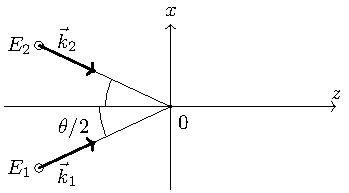
\includegraphics[scale=1.5]{fig/fig1.pdf}
	\caption{Две волны в среде}
	\label{fig:figure1}
\end{figure}

Рассмотрим распространение двух плоских монохроматических волн
\begin{equation}
	\label{eq:pdv.1}
	\vec{E}_{1,2}=\operatorname{Re}\left\{\vec{y}_{0} \tilde{E}_{1,2}(z) \cdot \exp \left[i\left(-k_{z} z \mp k_{x} x+\omega t\right)\right]\right\}
\end{equation}
в однородном изотропном полупространстве $z>0$ (Рис. \ref{fig:figure1}) движущейся с постоянной скоростью $v_0 \vec{x}_0$ жидкой (или газообразной) среды, имеющей линейную диэлектрическую проницаемость $\varepsilon_0$ и проводимость $\sigma_0$. Падающие из вакуума на границу среды волны поляризованы перпендикулярно плоскости падения. Внутри среды их волновые векторы $\vec{k}_{1,2} = \pm k_x \vec{x}_0 + k_z \vec{z_0}$, направленные симметрично относительно оси OZ, имеют составляющие
\begin{equation}
	\label{eq:pdv.2}
	k_{x}=k_{0} \sin (\theta / 2) \equiv(\omega / c) \sin (\theta / 2) ; \quad k_{z}=\sqrt{k_{0}^{2} \varepsilon_{0} \mu-k_{x}^{2}} \equiv \sqrt{k^{2}-k_{x}^{2}}.
\end{equation}
Трансформация комплексной амплитуды поля в среде описывается скалярным волновым уравнением Гельмгольца
\begin{equation}
	\label{eq:pdv.3}
	\Delta \tilde{E}+k^{2} \tilde{E}-\frac{i \omega}{c^{2}} \mu 4 \pi \sigma_{0} \tilde{E}=-\omega^{2} \mu \frac{4 \pi}{c^{2}} \tilde{P}^\text{nl},
\end{equation}
где $\sigma_{0}$ - проводимость среды, $\mu$ - магнитная проницаемость, $\tilde{P}^\text{nl}$ - комплексная амплитуда нелинейной поляризации среды (предполагается, что $\vec{P}^\text{nl} \upuparrows \vec{E}$).

За счет пространственно неоднородного тепловыделения в интерференционном поле $\overline{|\vec{E}|}^{({2\pi}/{\omega})}$ двух разнонаправленных волн в проводящей среде возникает тепловая решетка с периодом $\Lambda = \pi / k_x$, равным периоду интерференционной картины. Тепловая решетка формирует нелинейную поляризацию среды
\begin{equation}
	\label{eq:pdv.4}
	\tilde{P}^\text{nl}=\frac{\delta \varepsilon}{4 \pi} \tilde{E}
\end{equation}
и тем самым создаёт нелинейную часть $\delta \varepsilon$ её диэлектрической проницаемости $\varepsilon = \varepsilon_0 + \delta\varepsilon$.


\subsection{Модель теплового механизма нелинейности}
Как известно, все процессы и все движения в жидкости (или газе) описываются уравнениями гидродинамики. Они отражают законы сохранения массы, импульса и энергии элементарной жидкой частицы и в наиболее общем случае могут быть представлены в виде системы трёх уравнений
\begin{equation}
	\label{eq:pdv.5}
	\frac{\partial \rho}{\partial t}+\operatorname{div}(\rho \vec{v})=0,
\end{equation}
\begin{equation}
	\label{eq:pdv.6}
	\frac{\partial \vec{v}}{\partial t}+(\vec{v} \cdot \nabla) \vec{v}=-\frac{\nabla p}{\rho}+\vec{g}-\frac{\nabla V}{\rho}+\frac{\operatorname{div} \hat{\sigma}}{\rho},
\end{equation}
\begin{equation}
	\label{eq:pdv.7}
	\rho T\left[\frac{\partial S}{\partial t}+(\vec{v} \cdot \nabla S)\right]=(\hat{\sigma} \cdot \nabla) \vec{v}+\operatorname{div}(\kappa \nabla T)+\overline{\Pi}^{(2 \pi / \omega)},
\end{equation}
в которых $\rho$ - плотность среды, $p$ - давление, $\vec{v}$ - скорость движения элементарного объёма жидкости, $T$ - температура, $S$ - энтропия, $\vec{g}$ - ускорение свободного падения, $\kappa$ - коэффициент теплопроводности среды,
\begin{equation}
	\label{eq:pdv.8}
	\overline{\Pi}^{(2 \pi / \omega)}=\sigma_{0} \overline{|\vec{E}|^{2}}^{(2 \pi / \omega)}-\left[\frac{T}{8 \pi}\left(\frac{\partial \varepsilon}{\partial T}\right)_{p}\right]_{0} \frac{\partial}{\partial T} \overline{|\vec{E}|^{2}}^{(2 \pi / \omega)}
\end{equation}
-- мощность индуцированных полем источников тепла (второе слагаемое учитывает электрокалорический эффект), $\hat{\sigma}$ - тензор вязких напряжений, связанный со скоростью дифференциальным соотношением
\begin{equation}
	\label{eq:pdv.9}
	\operatorname{div} \hat{\sigma}=\eta \Delta \vec{v}+[(\eta / 3)+\zeta](\nabla \cdot \operatorname{div} \vec{v}),
\end{equation}
где $\eta$, $\zeta$ - коэффициенты вязкости,
\begin{equation}
	\label{eq:pdv.10}
	V=-\frac{1}{8 \pi}\left(\rho \frac{\partial \varepsilon}{\partial \rho}\right)_{S} \overline{|\vec{E}|^{2}}^{(2 \pi / \omega)}
\end{equation}
-- потенциальная энергия электрострикции. Система материальных уравнений \eqref{eq:pdv.5} -- \eqref{eq:pdv.7} включает в себя также уравнение состояния среды, которое может связывать любые три величины из полного набора переменных термодинамических величин и зависит от условий эксперимента. В частности, уравнение состояния среды может иметь одну из возможных форм
\begin{equation}
	\label{eq:pdv.11}
	\rho=f_{1}(p, T) ; \quad S=f_{2}(p, T).
\end{equation}
Система материальных уравнений \eqref{eq:pdv.5} - \eqref{eq:pdv.7} и \eqref{eq:pdv.11} совместно с уравнением Гельмгольца \eqref{eq:pdv.3} для электромагнитного поля является замкнутой и полной для описания взаимодействия монохроматического лазерного излучения с жидкой нелинейной средой. В разных (по химическому составу) средах и в различных экспериментальных условиях отдельные компоненты материальных уравнений могут вносить пренебрежимо малые вклады в описание нелинейных явлений. В частности, при описании стационарного ПДВ можно не учитывать вклада в нагревание среды электрокалорического эффекта \eqref{eq:pdv.8}. Учитывая, что характерное время формирования нелинейной поляризации намного больше времени, за которое звуковая волна успевает пробежать период возникающей в среде тепловой решетки и выровнять давление в среде, можно и нужно пренебречь энергией электрострикции \eqref{eq:pdv.10}, т.е. третьим членом в правой части уравнения \eqref{eq:pdv.6}.

В практически реализуемых условиях жидкость (или газ) оказывается средой со слабой нелинейностью, и воздействие лазерного излучения на такую среду проявляется в виде весьма малых отклонений термодинамических величин $\rho$, $p$, $S$, $T$, $\vec{v}$ от их стационарных невозмущенных значений. Поэтому почти все регистрируемые нелинейные эффекты, включая ПДВ, с большой точностью можно описывать материальными уравнениями для возмущений термодинамических величин среды.


Считая возмущения $\tilde{\rho}$, $\tilde{p}$, $\tilde{S}$, $\tilde{T}$, $\vec{\tilde{v}}$, вносимые полем в среду, малыми по сравнению с невозмущёнными стационарными значениями $\rho_0$, $p_0$, $S_0$, $T_0$, $\vec{v}_0$, вначале линеаризуем уравнения \eqref{eq:pdv.5}, \eqref{eq:pdv.6} и преобразуем их в уравнения
\begin{equation}
	\label{eq:pdv.12}
	\frac{\partial \tilde{\rho}}{\partial t}+\operatorname{div}\left(\rho_{0} \vec{\tilde{v}}\right)+\operatorname{div}\left(\tilde{\rho} \vec{v}_{0}\right)=0,
\end{equation}
\begin{equation}
	\label{eq:pdv.13}
	\rho_{0}\left(\frac{\partial \vec{\tilde{v}}}{\partial t}\right)+\rho_{0}\left(\vec{v}_{0} \cdot \nabla\right) \vec{v}=-\nabla \tilde{p}+\frac{1}{\rho_{0}}\left\{\eta \Delta \rho_{0} \vec{v}+[(\eta / 3)+\zeta] \nabla \operatorname{div}\left(\rho_{0} \vec{v}\right)\right\}.	
\end{equation}
Применим операцию дивергенции к уравнению \eqref{eq:pdv.13} и, используя \eqref{eq:pdv.12} в виде
\begin{equation}
	\label{eq:pdv.12'}
	\operatorname{div}\left(\rho_{0} \vec{\tilde{v}}\right)=-\frac{\partial \tilde{\rho}}{\partial t}-\left(\vec{v}_{0} \cdot \nabla \tilde{\rho}\right),
\end{equation}
получим уравнение
\begin{equation}
	\label{eq:pdv.14}
	\left[\frac{\partial}{\partial t}+\left(\vec{v}_{0} \cdot \nabla\right)-\frac{1}{\rho_{0}}\left(\frac{4 \eta}{3}+\zeta\right) \Delta\right]\left\{\frac{\partial \tilde{\rho}}{\partial t}+\left(\vec{v}_{0} \cdot \nabla \tilde{\rho}\right)\right\}=\Delta \tilde{p},
\end{equation}
которое связывает изменения плотности среды $\tilde{\rho}$ и давления в ней $\tilde{p}$.

Поскольку экспериментально измеряются изменения давления и температуры, то уравнение \eqref{eq:pdv.14} следует трансформировать так, чтобы оно описывало связь возмущений термодинамических величин $p$ и $T$. Это нетрудно сделать, используя одно из возможных уравнений состояния среды, связывающее плотность, давление и температуру. Линеаризуя первое уравнение \eqref{eq:pdv.11} вблизи состояния равновесия, получим связь между изменениями плотности, давления и температуры
\begin{equation}
	\label{eq:pdv.15}
	\tilde{\rho}=\left(\frac{\partial f_{1}}{\partial p}\right)_{p_{0}, T_{0}} \tilde{p}+\left(\frac{\partial f_{1}}{\partial T}\right)_{p_{0}, T_{0}} \tilde{T},
\end{equation}
которая позволяет (путём исключения $\tilde{\rho}$) преобразовать \eqref{eq:pdv.14} в уравнение
\begin{equation}
	\label{eq:pdv.16}
	\begin{array}{l}
	\left(\frac{\partial f_{1}}{\partial p}\right)_{p_{0}, T_{0}}\left[\frac{\partial}{\partial t}+\left(\vec{v}_{0} \cdot \nabla\right)-\frac{1}{\rho_{0}}\left(\frac{4 \eta}{3}+\zeta\right) \Delta\right]\left\{\frac{\partial \tilde{p}}{\partial t}+\left(\vec{v}_{0} \cdot \nabla \tilde{p}\right)\right\}-\Delta \tilde{p}+ \\
	+\left(\frac{\partial f_{1}}{\partial T}\right)_{p_{0}, T_{0}}\left\{\frac{\partial}{\partial t}+\left(\vec{v}_{0} \cdot \nabla\right)-\frac{1}{\rho_{0}}\left(\frac{4 \eta}{3}+\zeta\right) \Delta\right\}\left[\frac{\partial \tilde{T}}{\partial t}+\left(\vec{v}_{0} \cdot \nabla \tilde{T}\right)\right]=0
\end{array}
\end{equation}
относительно возмущений давления и температуры. Эксперимент проводится в условиях постоянного давления ($p = \mathrm{const} = p_0 $), когда все переходные процессы завершены и потому отсутствуют вариации давления ($\tilde{p}=0$). Поэтому \eqref{eq:pdv.16} приобретает вид уравнения
\begin{equation}
	\label{eq:pdv.17}
	\left\{\frac{\partial^{2}}{\partial t^{2}}+\frac{\partial}{\partial t}\left(\vec{v}_{0} \cdot \nabla\right)+\left(\vec{v}_{0} \cdot \nabla\right)^{2}-\frac{1}{\rho_{0}}\left(\frac{4 \eta}{3}+\zeta\right) \Delta\left[\frac{\partial}{\partial t}+\left(\vec{v}_{0} \cdot \nabla\right)\right]\right\} \tilde{T}=0,
\end{equation}
в котором отсутствуют источники для роста температуры. Это означает, что материальные уравнения \eqref{eq:pdv.5} и \eqref{eq:pdv.6} не вносят никакого вклада в тепловую нелинейность проводящей среды.

Обратимся к материальному уравнению \eqref{eq:pdv.7}, которое является следствием закона сохранения энергии элементарного объёма среды. Линеаризуя \eqref{eq:pdv.7} вблизи стационарных значений термодинамических величин, получим уравнение
\begin{equation}
	\label{eq:pdv.18}
	\rho_{0} T_{0}\left[\frac{\partial \tilde{S}}{\partial t}+\left(\vec{v}_{0} \cdot \nabla \tilde{S}\right)\right]=(\hat{\sigma} \cdot \nabla) \vec{\tilde{v}}+\operatorname{div}(\kappa \nabla \tilde{T})+\sigma_{0} \overline{|\vec{E}|^{2}}^{(2\pi/\omega)},
\end{equation}
описывающее изменения энтропии и температуры. Поскольку тепловыделение, обусловленное внутренним трением, пропорционально членам второго порядка малости по возмущению скорости $\vec{\tilde{v}}$ и практически ничтожно мало по сравнению с тепловыделением при поглощении, то число членов в правой части \eqref{eq:pdv.18} можно и нужно уменьшить до двух, избавившись от $(\hat{\sigma} \cdot \nabla)\vec{\tilde{v}}$.

Уравнение \eqref{eq:pdv.18} следует преобразовать в уравнение, связывающее возмущения давления и температуры. Для этого необходимо использовать другую линеаризованную форму уравнения \eqref{eq:pdv.11} состояния среды
\begin{equation}
	\label{eq:pdv.19}
	\tilde{S}=\left(\frac{\partial f_{2}}{\partial p}\right)_{p_{0}, T_{0}} \tilde{p}+\left(\frac{\partial f_{2}}{\partial T}\right)_{p_{0}, T_{0}} \tilde{T}.
\end{equation}
Подставляя \eqref{eq:pdv.19} в \eqref{eq:pdv.18}, получим уравнение для возмущений давления и температуры
\begin{equation}
	\label{eq:pdv.20}
	\rho_{0} C_{p}\left[\frac{\partial \tilde{T}}{\partial t}+\left(\vec{v}_{0} \cdot \nabla \tilde{T}\right)\right]+\rho_{0} T_{0}\left[\frac{\partial \tilde{p}}{\partial t}+\left(\vec{v}_{0} \cdot \nabla \tilde{p}\right)\right] \cdot\left(\frac{\partial \tilde{S}}{\partial \tilde{p}}\right)_{T}=\kappa \Delta \tilde{T}+\sigma_{0} \overline{|\vec{E}|^{2}}^{(2 \pi / \omega)},
\end{equation}
в котором использовано понятие теплоёмкости при постоянном давлении $C_p = T_0 (\partial S  / \partial T)_p  = T_0 (\partial f_2  / \partial T)_p$. При условии $p = \mathrm{const} = p_0 $ ($\tilde{p}=0$) уравнение \eqref{eq:pdv.20} трансформируется в уравнение для температуры
\begin{equation}
	\label{eq:pdv.21}
	\left[\frac{\partial \tilde{T}}{\partial t}+\left(\vec{v}_{0} \cdot \nabla \tilde{T}\right)\right]-\chi \Delta \tilde{T}=\frac{\sigma_{0}}{\rho_{0} C_{p}} \overline{|\vec{E}|^{2}}^{(2 \pi / \omega)},
\end{equation}
которое описывает изменение $\tilde{T}$ в среде, имеющей коэффициент температуропроводности
\begin{equation}
	\label{eq:pdv.22}
	\chi=\left(\kappa / \rho_{0} C_{p}\right).
\end{equation}
Источником температуры в правой части \eqref{eq:pdv.21} являются тепловые потери в проводящей среде. Температуропроводность среды -- это следствие потока тепла из-за наличия градиента температуры.



\subsection{Стационарное взаимодействие двух попутных волн}

В общем случае для корректного решения уравнения \eqref{eq:pdv.21} необходимо задать граничные и начальное условия. В случае ПДВ из-за отсутствия конкретных сведений о форме и температуре поверхности трубы, в которой течёт жидкость, граничные условия для уравнения теплопроводности можно учесть приближенно. Для этого достаточно ввести в его левую часть дополнительный член $\tilde{T} / \tau_0$, формально учитывающий теплообмен с окружающей средой. 
Феноменологически вводимую в уравнение \eqref{eq:pdv.21} величину $\tau_0^{-1}$ называют коэффициентом потери температуры в результате теплоотвода.

Начальное условие необходимо для описания процесса изменения
температуры текущей жидкости $\tilde{T}(t)$ во времени, например, с целью изучения механизмов формирования ПДВ. В этом случае начальным условием было бы естественно считать $\tilde{T}(t=0) = 0$. Для описания стационарного ПДВ, когда процесс изменения температуры прекратился и можно положить $(\partial \tilde{T}  / \partial t) = 0$, начальное условие оказывается излишним.

Малая нелинейная часть диэлектрической проницаемости $\delta \varepsilon$, которая образуется в проводящей среде из-за изменения температуры и давления, в общем случае может быть представлена в виде
\begin{equation}
	\label{eq:pdv.23}
	\delta \varepsilon=\left(\frac{\partial \varepsilon}{\partial T}\right)_{p} \tilde{T}+\left(\frac{\partial \varepsilon}{\partial p}\right)_{T} \tilde{p}.
\end{equation}
В установившемся (стационарном) режиме ПДВ, когда $p=\mathrm{const}$ и $\tilde{p} = 0$, образовавшаяся в проводящей среде нелинейная часть диэлектрической проницаемости $\delta \varepsilon$ с точностью до постоянного коэффициента совпадает с возмущением температуры $\tilde{T}$:
\begin{equation}
	\label{eq:pdv.24}
	\delta \varepsilon=(\partial \varepsilon / \partial T)_{p} \tilde{T}.
\end{equation}
Таким образом, в стационарном случае с учётом потери температуры из-за теплоотвода и с помощью \eqref{eq:pdv.24} уравнение \eqref{eq:pdv.21} преобразуется в уравнение
\begin{equation}
	\label{eq:pdv.25}
	\frac{\delta \varepsilon}{\tau_{0}}+\left(\overrightarrow{v}_{0} \cdot \nabla \delta \varepsilon\right)-\frac{\kappa}{\rho_{0} C_{p}} \Delta \delta \varepsilon=\frac{\sigma_{0}}{\rho_{0} C_{p}} \cdot\left(\frac{\partial \varepsilon}{\partial T}\right)_{p} \overline{|\vec{E}|^{2}}^{(2 \pi / \omega)}
\end{equation}
относительно нелинейной диэлектрической проницаемости $\delta \varepsilon$. Её пространственная структура формируется средней за период $(2 \pi / \omega)$ интенсивностью
\begin{equation}
	\label{eq:pdv.26}
	\overline{|\vec{E}|^{2}}^{(2 \pi / \omega)}=\frac{1}{2} \cdot\left\{\left|\tilde{E}_{1}(z)\right|^{2}+\left|\tilde{E}_{2}(z)\right|^{2}+\left[\tilde{E}_{1}(z) \tilde{E}_{2}^{*}(z) \exp \left(-i 2 k_{x} x\right)+\text{ к. с.}\right]\right\}
\end{equation}
интерференционного поля $\vec{E}$ двух волн с медленно меняющимися вдоль координаты $z$ комплексными амплитудами $\tilde{E}_{1,2}(z)$. Изменение комплексной амплитуды поля $\tilde{E}$ описывается скалярным уравнением Гельмгольца \eqref{eq:pdv.3}, которое с учётом \eqref{eq:pdv.2} и \eqref{eq:pdv.4} приобретает форму
\begin{equation}
	\label{eq:pdv.27}
	\Delta \tilde{E}+k^{2} \tilde{E}-i k^{2} \frac{4 \pi \sigma_{0}}{\varepsilon_{0} \omega} \tilde{E}=-k^{2} \frac{\delta \varepsilon}{\varepsilon_{0}} \tilde{E}.
\end{equation}
Уравнения \eqref{eq:pdv.25} и \eqref{eq:pdv.27} образуют замкнутую систему. Анализ этой пары уравнений позволяет вполне однозначно определить пространственную структуру нелинейной диэлектрической проницаемости в виде
\begin{equation}
	\label{eq:pdv.28}
	\delta \varepsilon=\delta \varepsilon^{\prime \prime}(z)+\left[\delta \tilde{\varepsilon}(z) \cdot \frac{1}{2} \cdot \exp \left(-2 i k_{x} x\right)+\text{ к. с.}\right],
\end{equation}
где средняя составляющая $\delta \varepsilon'' (z)$  и комплексная амплитуда $\delta \tilde{\varepsilon}$ решётки $\delta \varepsilon$ по координате $x$ являются медленно меняющимися на длине волны $\lambda = 2\pi / k$ функциями координаты $z$.

Подставляя \eqref{eq:pdv.28} в \eqref{eq:pdv.25} и используя ортогональность пространственных гармоник $\delta \varepsilon$ по координате $x$, нетрудно получить уравнения для средней составляющей   $\delta \varepsilon'' (z)$ и комплексной амплитуды $\delta \tilde{\varepsilon}$ решётки нелинейной диэлектрической проницаемости
\begin{equation}
	\label{eq:pdv.29}
	\frac{1}{\tau_{0}} \delta \varepsilon^{\prime \prime}(z) \cong \frac{\sigma_{0}}{2 \rho_{0} C_{p}}\left(\frac{\partial \varepsilon}{\partial T}\right)_{p}\left(\left|\tilde{E}_{1}\right|^{2}+\left|\tilde{E}_{2}\right|^{2}\right),
\end{equation}
\begin{equation}
	\label{eq:pdv.30}
	\left[-i {v}_{0} 2 k_{x}+\frac{\kappa 4 k_{x}^{2}}{\rho_{0} C_{p}}+\frac{1}{\tau_{0}}\right] \delta 
	\tilde{\varepsilon}(z) \cong \frac{\sigma_{0}}{\rho_{0} C_{p}} \cdot\left(\frac{\partial \varepsilon}{\partial T}\right)_{p} \tilde{E}_{1} \tilde{E}_{2}^{*}.
\end{equation}
При выводе \eqref{eq:pdv.29} и \eqref{eq:pdv.30} опущены малые члены ($d^2 \delta \varepsilon'' (z) / d z^2$) и ($d^2 \delta \tilde\varepsilon (z) / d z^2$)‚ что и определяет приближённый характер этих уравнений.

Подставляя поле $\tilde{E}$ в виде суммы волн \eqref{eq:pdv.1} в уравнение Гельмгольца \eqref{eq:pdv.27}
и используя ортогональность их полей по координате $x$ ‚ можно получить систему из двух связанных уравнений для комплексных амплитуд $\tilde{E}_{1,2}(z)$
\begin{equation}
	\label{eq:pdv.31}
	-2 i k_{z} \frac{\partial \tilde{E}_{1}}{\partial z}-i k^{2} \frac{4 \pi \sigma_{0}}{\varepsilon_{0} \omega} \tilde{E}_{1} \cong-\frac{k^{2}}{\varepsilon_{0}}\left\{\delta \varepsilon^{\prime \prime} \cdot \tilde{E}_{1}+\frac{1}{2} \delta \tilde{\varepsilon} \cdot \tilde{E}_{2}\right\},
\end{equation}
\begin{equation}
	\label{eq:pdv.32}
	-2 i k_{z} \frac{\partial \tilde{E}_{2}}{\partial z}-i k^{2} \frac{4 \pi \sigma_{0}}{\varepsilon_{0} \omega} \tilde{E}_{2} \cong-\frac{k^{2}}{\varepsilon_{0}}\left\{\delta \varepsilon^{\prime \prime} \cdot \tilde{E}_{2}+\frac{1}{2} \delta \tilde{\varepsilon}^{*} \cdot \tilde{E}_{1}\right\},
\end{equation}
из которых исключены как ничтожно малые члены ($d^2 \tilde{E}_{1,2} / dz^2$).

Уравнения \eqref{eq:pdv.29} -- \eqref{eq:pdv.32} образуют систему с большим числом коэффициентов разной размерности, что препятствует выявлению физической природы и
оценкам величин основных параметров механизма ПДВ. С целью упрощения
записи уравнений целесообразно ввести безразмерные амплитуды волн поля
\begin{equation}
	\label{eq:pdv.33}
	\tilde{\mathcal{E}}_{1,2}=\left(\tilde{E}_{1,2} / \sqrt{\left|\tilde{E}_{1}(0)\right|^{2}}\right) \equiv\left(\tilde{E}_{1,2} / \sqrt{I_{0}}\right)
\end{equation}
и их интенсивности 
\begin{equation}
	\label{eq:pdv.34}
	\tilde{\mathcal{E}}_{1,2} \cdot \tilde{\mathcal{E}}_{1,2}^* \equiv \mathcal{E}_{1,2}^{2},
\end{equation}
безразмерную координату
\begin{equation}
	\label{eq:pdv.35}
	\xi = z \cdot \frac{k^2}{k_z \varepsilon_0},
\end{equation}
безразмерный коэффициент затухания поля в проводящей среде
\begin{equation}
	\label{eq:pdv.36}
	\gamma = \frac{4\pi \sigma_0}{\omega}
\end{equation}
и следующие физические параметры: обусловленное коэффициентами теплоотвода $1/\tau_0$ и температуропроводности ($\chi = [\kappa / \rho_0 C_p]$) среды время
\begin{equation}
	\label{eq:pdv.37}
	\tau_\text{r} = \frac{\tau_0}{1+4\chi k_x^2 \tau_0},
\end{equation}
имеющее смысл времени релаксации решётки диэлектрической проницаемости
при описании нестационарного ПДВ, безразмерный параметр
\begin{equation}
	\label{eq:pdv.38}
	\delta = v_0 2 k_x \tau_\text{r},
\end{equation}
определяющий величину пространственного смещения решётки диэлектрической проницаемости относительно интерференционной картины распределения
интенсивности поля в среде, безразмерный параметр нелинейности среды
\begin{equation}
	\label{eq:pdv.39}
	G = \frac{\sigma_0 \tau_\text{r} I_0}{4 \varepsilon_0 \rho_0 C_p} \left(\frac{\partial \varepsilon}{\partial T}\right)_p,
\end{equation}
характеризующий эффективность ПДВ. В безразмерном виде уравнения \eqref{eq:pdv.29} -- \eqref{eq:pdv.32} примут компактную форму
\begin{equation}
	\label{eq:pdv.40}
	\delta \varepsilon^{\prime \prime}=2 G\left(\tau_{0} / \tau_{\mathrm{r}}\right) \cdot\left({\mathcal { E }}_{1}^{2}+\mathcal{E}_{2}^{2}\right), 
\end{equation}
\begin{equation}
	\label{eq:pdv.41}
	\delta \tilde{\varepsilon}=\frac{4 G}{1+i \delta} \cdot \tilde{\mathcal{E}}_{1} \tilde{\mathcal{E}}_{2}^{*},
\end{equation}
\begin{equation}
	\label{eq:pdv.42}
	\left[\frac{d}{d \xi}+\frac{\gamma}{2}\right] \tilde{\mathcal{E}}_{1}=\frac{-i}{2} \cdot\left(\delta \varepsilon^{\prime \prime} \cdot \tilde{\mathcal{E}}_{1}+\frac{1}{2} \delta \tilde{\varepsilon} \cdot \tilde{\mathcal{E}}_{2}\right),
\end{equation}
\begin{equation}
	\label{eq:pdv.43}
	\left[\frac{d}{d \xi}+\frac{\gamma}{2}\right] \tilde{\mathcal{E}}_{2}=\frac{-i}{2} \cdot\left(\delta \varepsilon^{\prime \prime} \cdot \tilde{\mathcal{E}}_{2}+\frac{1}{2} \delta \tilde{\varepsilon}^{*} \cdot \tilde{\mathcal{E}}_{1}\right).
\end{equation}

Подставляя выражения $\delta \varepsilon'' (z)$ из \eqref{eq:pdv.40} и $\delta \tilde{\varepsilon}$ из \eqref{eq:pdv.41} в \eqref{eq:pdv.42} и \eqref{eq:pdv.43}, нетрудно получить два связанных симметричных уравнения 
\begin{equation}
	\label{eq:pdv.44}
	\left[\frac{d}{d \xi}+\frac{\gamma}{2}+i 2 G \frac{\tau_{0}}{\tau_{\mathrm{r}}} \cdot\left({\mathcal { E }}_{1}^{2}+{\mathcal { E }}_{2}^{2}\right)\right] \tilde{\mathcal{E}_{1}}=\frac{-i G}{1+i \delta} \cdot \mathcal{E}_{2}^{2} \tilde{\mathcal{E}}_{1},
\end{equation}
\begin{equation}
	\label{eq:pdv.45}
	\left[\frac{d}{d \xi}+\frac{\gamma}{2}+i 2 G \frac{\tau_{0}}{\tau_{\mathrm{r}}} \cdot\left({\mathcal { E }}_{1}^{2}+{\mathcal { E }}_{2}^{2}\right)\right] \tilde{\mathcal{E}}_{2}=\frac{-i G}{1-i \delta} \cdot \mathcal{E}_{1}^{2} \tilde{\mathcal{E}}_{2}
\end{equation}

относительно амплитуд $\tilde{\mathcal{E}}_{1,2}$ взаимодействующих между собой волн. Механизмом взаимодействия является дифракция (или рассеяние) волн на решётке диэлектрической проницаемости среды. Механизм взаимодействия волн и пределы его возможностей становятся более понятными, если от \eqref{eq:pdv.44} и \eqref{eq:pdv.45} перейти к уравнениям для интенсивностей ${\mathcal{E}}_{1,2}^2$.


Уравнения для интенсивностей взаимодействующих волн
\begin{equation}
	\label{eq:pdv.46}
	{\left[\frac{d}{d \xi}+\gamma \right] \mathcal{E}_{1}^{2}=\frac{-2 \delta G}{1+\delta^{2}} \cdot \mathcal{E}_{2}^{2} \mathcal{E}_{1}^{2}},
\end{equation}
\begin{equation}
	\label{eq:pdv.47}
	\left[\frac{d}{d \xi}+\gamma \right] \mathcal{E}_{2}^{2}=\frac{2 \delta G}{1+\delta^{2}} \cdot \mathcal{E}_{1}^{2} \mathcal{E}_{2}^{2}
\end{equation}
имеют одинаковые по величине и противоположные по знаку правые части. Это значит, что в случае
\begin{equation*}
	\delta G > 0
\end{equation*}
интенсивность волны ${\mathcal{E}}_{2}^2$ будет приобретать дополнительную энергию в результате рассеяния на решётке $\delta \varepsilon$ в направлении $\vec{k}_2$ взаимодействующей с ней и теряющей свою энергию первой волны. Если дополнительная энергия $2\delta G \cdot \mathcal{E}_1^2 \cdot \mathcal{E}_2^2 / (1+\delta^2)$, которую получает вторая волна от первой, будет больше энергии $\gamma \mathcal{E}_2^2$, которую она теряет из-за наличия линейного поглощения, то интенсивность $\mathcal{E}_2^2$ будет расти. Наибольшая эффективность перекачки энергии при прочих равных условиях будет иметь место при $|\delta| = 1$, и, следовательно, оптимальная скорость течения среды составляет
\begin{equation}
	\label{eq:pdv.48}
	(v_0)_\text{opt} = \frac{1}{2 k_x \tau_\text{r}}.
\end{equation}
При этом интенсивность $\mathcal{E}_1^2$ волны-донора согласно \eqref{eq:pdv.44} монотонно уменьшается. Т.e., условие роста интенсивности $\mathcal{E}_2^2$ волны-акцептора
\begin{equation}
	\label{eq:pdv.49}
	2 \delta G \cdot \mathcal{E}_{1}^{2} /\left(1+\delta^{2}\right)>\gamma
\end{equation}
по мере продвижения вглубь слоя среды выполняется с монотонно уменьшающимся запасом прочности. В некотором сечении $\xi_\text{cr}$ слоя среды неравенство \eqref{eq:pdv.49} превращается в равенство, и именно в этом сечении, где
\begin{equation}
	\label{eq:pdv.50}
	\left({\mathcal { E }}_{1}^{2}\right)_\text{cr}=\gamma \cdot\left(1+\delta^{2}\right) / 2 \delta G,
\end{equation}
волна-акцептор достигает своей максимальной интенсивности. Затем из-за уменьшения интенсивности $\mathcal{E}_1^2$ волны-донора знак неравенства становится противоположным, и интенсивность $\mathcal{E}_2^2$ начинает уменьшаться. Уравнения \eqref{eq:pdv.46}, \eqref{eq:pdv.47} имеют точные решения, которые позволяют проследить изменение интенсивностей $\mathcal{E}_{1,2}^2$ вдоль направления оси OZ.

Получим явные выражения зависимостей $\mathcal{E}_{1,2}^2 (\xi)$. Для этого произведем замену переменных и координаты по формулам
\begin{equation}
	\label{eq:pdv.51}
	\mathcal{E}_{1,2}^{2}(\xi)=\{W(y), U(y)\} \cdot \exp (-\gamma \xi),
\end{equation}
\begin{equation}
	\label{eq:pdv.52}
	y=\frac{2 \delta G}{1+\delta^{2}}[1-\exp (-\gamma \xi)] \cdot \frac{1}{\gamma}.
\end{equation}
Новые функции $\{W(y), U(y)\}$ будут удовлетворять системе уравнений
\begin{equation}
	\label{eq:pdv.53}
	\frac{d W}{dy} = - UW,
\end{equation}
\begin{equation}
	\label{eq:pdv.54}
	\frac{d U} {du} = UW,
\end{equation}
которая имеет первый интеграл
\begin{equation}
	\label{eq:pdv.55}
	W+U=\text {const}=W(0)+U(0) \equiv \mathcal{E}_{1}^{2}(0)+\mathcal{E}_{2}^{2}(0) \equiv 1+R,
\end{equation}
где $R$ - отношение интенсивности $\mathcal{E}_{2}^{2}(0)$ к интенсивности $\mathcal{E}_{1}^{2}(0) = 1$ на входе слоя среды. Интеграл \eqref{eq:pdv.55} позволяет представить систему \eqref{eq:pdv.53}, \eqref{eq:pdv.54} в виде одного из двух независимых друг от друга и полностью эквивалентных друг другу уравнений 
\begin{equation}
	\label{eq:pdv.56}
	\frac{d U}{d y}=U(1+R-U) ; \quad \frac{d W}{d y}=-W(1+R-W).
\end{equation}
Каждое из решений
\begin{equation}
	\label{eq:pdv.57}
	W(y)=\frac{(1+R) \cdot \exp [-(1+R) y]}{R+\exp [-(1+R) y]} ; \quad U(y)=\frac{R \cdot(1+R)}{R+\exp [-(1+R) y]}
\end{equation}
уравнений \eqref{eq:pdv.56} совместно с первым интегралом \eqref{eq:pdv.55} и выражением \eqref{eq:pdv.52} для координаты $y$ полностью описывает распределение интенсивностей двух волн
\begin{equation}
	\label{eq:pdv.58}
	\mathcal{E}_{1}^{2}(\xi)=\frac{(1+R) \cdot \exp (-\gamma \xi)}{R \exp [(1+R) y]+1} ; \quad \mathcal{E}_{2}^{2}(\xi)=\frac{R \cdot(1+R) \cdot \exp (-\gamma \xi)}{R+\exp [-(1+R) y]}
\end{equation}
в пространстве проводящей среды в случае стационарного ПДВ. В приближении очень слабого линейного затухания
\begin{equation}
	\label{eq:pdv.59}
	\gamma \xi \ll 1,
\end{equation}
когда координата
\begin{equation}
	\label{eq:pdv.60}
	y \cong\left(2 G \delta / \left[1+\delta^{2}\right]\right) \xi \equiv 2 \delta \tilde{G} \xi
\end{equation}
оказывается пропорциональной $\xi$, интенсивности \eqref{eq:pdv.58} приобретают вид
\begin{equation}
	\label{eq:pdv.61}
	\mathcal{E}_{1}^{2}(\xi)=\frac{(1+R) \cdot(1-\gamma \xi)}{R \cdot \exp [(1+R) \cdot 2 \delta \tilde{G} \xi]+1};\quad \mathcal{E}_{2}^{2}(\xi)=\frac{R \cdot(1+R) \cdot(1-\gamma \xi)}{R+\exp [-(1+R) 2 \delta \tilde{G} \xi]}.
\end{equation}
Результаты предоставленной теории стационарного ПДВ можно обобщить на случай, когда частоты взаимодействующих волн
\begin{equation}
	\label{eq:pdv.62}
	\vec{E}_{1,2}=\left\{\vec{y}_{0} \tilde{E}_{1,2} \cdot \exp \left[i\left(\omega \pm \frac{\Delta \omega}{2}\right) t-i\left(k_{z} z \pm k_{x} x\right)\right]\right\}
\end{equation}
отличаются друг от друга на величину $\Delta \omega \ll \omega$. В этом случае интерференционная картина волн $\tilde{E}_{1,2}$ будет <<бежать>> вдоль оси ОХ со скоростью
\begin{equation}
	\label{eq:pdv.63}
	v' = \frac{\Delta \omega}{2 k_x}.
\end{equation}
Если перейти в систему координат, движущуюся вместе с интерференционной картиной, то этот более общий случай сведется к ранее рассмотренному, только среда теперь будет двигаться относительно интерференционной картины со скоростью
\begin{equation}
	\label{eq:pdv.64}
	v = v_0 + v' = v_0 + \frac{\Delta \omega}{2 k_x}.
\end{equation}
Соответствующий безразмерный параметр будет иметь вид
\begin{equation}
	\label{eq:pdv.65}
	\delta = 2k_x v \tau_\text{r} = 2k_x v_0 \tau_\text{r} + \Delta \omega \tau_\text{r}.
\end{equation}
Из \eqref{eq:pdv.65} видно, что оптимальный энергообмен ($|\delta| = 1$) может быть достигнут и в покоящейся среде ($\vec{v}_0 = 0$) за счет сдвига на величину
\begin{equation}
	\label{eq:pdv.66}
	\Delta \omega_\text{opt} = \frac{1}{\tau_\text{r}}
\end{equation}
частот взаимодействующих волн.
%!TEX root = ../ltransform.tex
\section{Метод обращения волнового фронта излучения}

Одной из важнейших задач квантовой электроники является уменьшение угловой расходимости лазерного излучения, достижение минимальной дифракционной расходимости
\begin{equation}
	\Delta \theta = \frac{\lambda}{D},
\end{equation}
где $\Delta \theta$ - угловая ширина диаграммы направленности, $\lambda$ - длина волны и $D$ - характерный размер области источника излучения. Главная причина, по которой расходимость генерируемых лазерами полей превосходит дифракционную, состоит в том, что в оптических трактах лазерных устройств обычно присутствуют всевозможные неоднородности диэлектрической проницаемости, вносящие негативный вклад в структуру фазового фронта распространяющегося излучения. Поскольку техническое устранение даже небольшой части неоднородностей является крайне сложным, то чрезвычайно актуальными представляются исследования и разработки новых методов передачи энергии и информации в оптике, позволяющих обеспечить высокие выходные характеристики лазерного излучения. В литературе они получили наименование методов фазовой коррекции волновых фронтов излучения.

В настоящем параграфе мы обсудим одно замечательное явление нелинейной оптики, которое может быть использовано для устранения негативного влияния оптических неоднородностей на структуру распространяющихся электромагнитных полей. Это явление называется эффектом обращения волнового фронта (ОВФ) излучения.

\begin{figure}[ht]
	\centering
	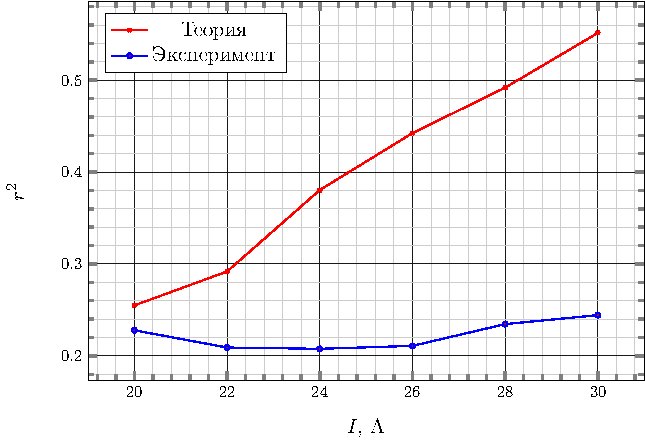
\includegraphics[scale=1.5]{fig/fig2.pdf}
	\caption{}
	\label{fig:figure2}
\end{figure}

Прежде всего, поясним идею эффекта ОВФ и метода коррекции, на нём основанного. Пусть на фотопластинку ГФ (Рис. \ref{fig:figure2}) падает волна сигнала $\vec{E}_3$ и когерентная с ней опорная волна $\vec{E}_1$. Картина интерференции полей записывается в фотослое. Фотопластинка обрабатывается так, что интерференционные неоднородности проявляются в виде модуляции её прозрачности для излучения на частоте, на которой была создана и записана интерференционная картина. Получается так называемая голограмма. Если она достаточно тонкая, то ее действие на восстанавливающую волну можно описать введением комплексного коэффициента пропускания $\tilde{\Pi}$ для амплитуды поля
\begin{equation}
	\label{eq:2.1}
\tilde{E}_{\tau}(\vec{r}\,)=\tilde{\Pi}(\vec{r}\,) \tilde{E}_{i}(\vec{r}\,),
\end{equation}
где $ \tilde{E}_{i}$  падающее на слой и $ \tilde{E}_{\tau}$ - прошедшее через слой поля.

В простейшем случае вариации $R$ связаны с изменениями интенсивности записываемого поля, так что голограмма-транспарант имеет прозрачность
\begin{equation}
	\label{eq:2.2}
	\tilde{\Pi}(\vec{r}\,)=\operatorname{const}_{0} \cdot\left\{\tilde{E}_{1} \tilde{E}_{3}^{*}+\text {к.c.}\right\} \equiv C_{0} \cdot\left\{\tilde{E}_{1} \tilde{E}_{3}^{*}+\text {к.c.}\right\}
\end{equation}
Если направлять на транспарант считывающую волну $\vec{\tilde{E}}_2$ так,
 чтобы она распространялась точно навстречу опорной волне ($\tilde{E}_2 \sim \tilde{E}_1^*$), то после прохождения волны $\vec{\tilde{E}}_2$ через
  голограмму в соответствии с соотношением \eqref{eq:2.1} за счет первого слагаемого в \eqref{eq:2.2} восстанавливается поле
\begin{equation}
	\label{eq:2.3}
	\tilde{E}_{4}(\vec{r}\,) \sim\left|\tilde{E}_{1}(\vec{r}\,)\right|^{2} \tilde{E}_{3}^{*}(\vec{r}\,),
\end{equation}
распространяющееся навстречу сигналу $\tilde{E}_3$ и при $|\vec{\tilde{E}}_1|^2 = \mathrm{const}_1 = E_0^2$ отвечающее точно обращённой к сигналу волне.

\begin{figure}[h]
	\centering
	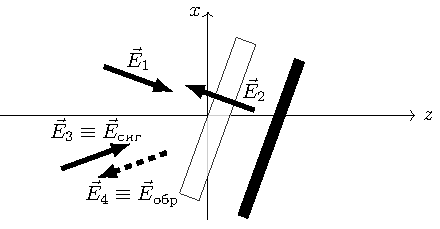
\includegraphics[scale=1.5]{fig/fig3.pdf}
	\caption{Волны $\vec{E}_{1,2}$ -- опорные, $\vec{E}_3$ -- сигнальная, $\vec{E}_4$ -- обращённая}
	\label{fig:figure3}
\end{figure}

Теперь представим себе, что для записи голограммы используется нелинейная среда (Рис. \ref{fig:figure3}) с диэлектрической проницаемостью
\begin{equation}
	\label{eq:2.4}
	\varepsilon=\varepsilon_{0}+\delta \varepsilon
	\left(
	\overline{{|\vec{E}|^{2}}}^{(2 \pi / \omega)}
	\right).
\end{equation}
В нелинейный слой одновременно направляются две опорных плоских волны
\begin{equation}
	\label{eq:2.5}
	\vec{E}_{1.2} =\operatorname{Re}\left\{\vec{\tilde{E}}_{1,2} \exp \left[i\left(\omega t \mp k_{z} z \pm k_{x} x\right)\right]\right\}
\end{equation}
и сигнальная волна
\begin{equation}
	\label{eq:2.6}
	\vec{E}_{3} =\operatorname{Re}\left\{\vec{\tilde{E}}_{3} \exp \left[i\left(\omega t-k_{z} z-k_{x} x\right)\right]\right\}.
\end{equation}
При этом вторая опорная плоская волна получается отражением первой от зеркала. В нелинейной среде \eqref{eq:2.4} процессы записи голографической решетки $(\delta \varepsilon)_{13} \sim \vec{\tilde{E}}_{1} \vec{\tilde{E}}_{3}^{*}+\text{к.с.}$ и ее считывания $(\delta \varepsilon )_{13} \cdot \vec{E}_2$ совмещены во времени.
Это -- динамическая голография. Динамическая голограмма обращает любую падающую сигнальную волну, автоматически подстраиваясь под нее. При этом обращенная волна
\begin{equation}
	\label{eq:2.7}
	\vec{\tilde{E}}_4 \sim \vec{\tilde{E}}_3^*
\end{equation}
возбуждается практически мгновенно, т.е. в реальном масштабе времени. Динамическую голограмму, обращающую волновой фронт падающего на нее излучения, называют ОВФ-зеркалом. Не трудно понять, как с помощью такого ОВФ-зеркала можно создать оптическую систему, способную скомпенсировать искажения сигнала (изображения) из-за наличия неоднородностей на трассе оптического пути внутри самого принимающего устройства.

\begin{figure}[ht]
	\centering
	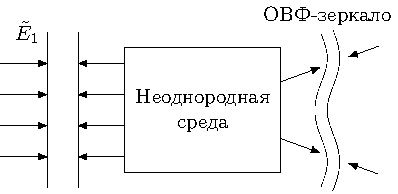
\includegraphics[scale=1.4]{fig/fig4.pdf}
	\caption{}
	\label{fig:figure4}
\end{figure}

Пусть плоская волна проходит через неоднородную среду, которая
искажает структуру её фазового фронта (Рис. \ref{fig:figure4}). На поверхность зеркала, которое должно формировать встречную волну, поступает поле
\begin{equation}
	\label{eq:2.8}
	\tilde{\Pi}(\vec{r}\,) \tilde{E}_{1} \sim \tilde{E}_{1} \exp [i \psi(\vec{r}\,)],
\end{equation}
где экспоненциальный множитель описывает влияние фазовых неоднородностей. С помощью обыкновенного зеркала можно сформировать отражённую волну, имеющую поле
\begin{equation}
	\label{eq:2.8'}
	\tilde{E}_{2} \sim \tilde{E}_{1} \exp [i \psi(\vec{r}\,)] \equiv \tilde{\Pi}(\vec{r}\,) \tilde{E}_{1}.
\end{equation}
Если рефлектором будет ОВФ-зеркало, то от него отразится поле
\begin{equation}
	\label{eq:2.9}
	\tilde{E}_{2} \sim \tilde{\Pi}^{*}(\vec{r}\,) \tilde{E}_{1}^{*} \equiv \tilde{E}_{1}^{*} \exp [-i \psi(\vec{r}\,)],
\end{equation}
которое после повторного прохождения волны через среду примет вид
\begin{equation}
	\label{eq:2.10}
	\tilde{E}_{3} \sim \tilde{E}_{2} \exp [i \psi(\vec{r}\,)] \sim \tilde{E}_{1}^{*}.
\end{equation}
\begin{figure}[hb]
	\centering
	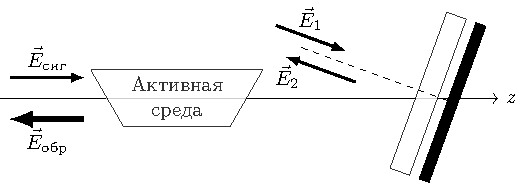
\includegraphics[scale=1.4]{fig/fig5.pdf}
	\caption{Волны $\vec{E}_{1,2}$ -- опорные, $\vec{E}_\text{сиг}\equiv\vec{E}_3$ -- сигнальная, $\vec{E}_\text{обр}\equiv\vec{E}_4$ -- обращённая}
	\label{fig:figure5}
\end{figure}
Таким образом, влияние фазовых неоднородностей будет ликвидировано. Если в качестве неоднородного материала взять активную среду, то получится двухпроходовый усилитель (Рис. \ref{fig:figure5}), фазовые неоднородности которого никак не влияют на усиливаемое излучение.





\subsection{ОВФ при четырёхволновом смешении в среде с тепловым механизмом нелинейности}

Важнейшей характеристикой ОВФ-зеркала, работающего в стационар­ном режиме, является комплексный коэффициент отражения
\begin{equation}
	\label{eq:2.11}
	\tilde{r}(0)=\frac{\tilde{\mathcal{E}}_{4}^{*}(0)}{\tilde{\mathcal{E}}_{3}(0)}.
\end{equation}
Чтобы найти эту величину для ОВФ-зеркала, выполненного на основе неподвижной ($\vec{v}_0 = 0$) проводящей ($\sigma_0$) среды с тепловым механизмом нелинейности, необходимо воспользоваться стационарными уравнениями для поля
\begin{equation}
	\label{eq:2.12}
	\Delta \tilde{E}+k^{2} \tilde{E}-i k^{2} \frac{4 \pi \sigma_{0}}{\varepsilon_{0} \omega} \tilde{E}=-k^{2} \frac{\delta \varepsilon}{\varepsilon_{0}} \tilde{E}
\end{equation}
и нелинейной диэлектрической проницаемости
\begin{equation}
	\label{eq:2.13}
	\frac{\delta \varepsilon}{\tau_{0}}-\chi \Delta \delta \varepsilon=\frac{\sigma_{0}}{\rho_{0} C_{p}} \cdot\left(\frac{\partial \varepsilon}{\partial T}\right)_{p} \overline{|\vec{E}|^{2}}^{(2\pi/\omega)}.
\end{equation}
Уравнение \eqref{eq:2.13} описывает структуру объёмных решёток $\delta \varepsilon$ индуцированных полем четырёх волн
\begin{equation}
	\label{eq:2.14}
	\begin{aligned}
	\tilde{E} &=\left[\tilde{E}_{1} \exp \left(i k_{x} x\right)+\tilde{E}_{3} \exp \left(-i k_{x} x\right)\right] \exp \left(-i k_{z} z\right)+\\
	&+\left[\tilde{E}_{2} \exp \left(-i k_{x} x\right)+\tilde{E}_{4} \exp \left(i k_{x} x\right)\right] \exp \left(i k_{z} z\right).
	\end{aligned}
\end{equation}
Две решётки записываются попутными волнами $\tilde{E}_1$, $\tilde{E}_3$, и $\tilde{E}_2$, $\tilde{E}_4$, ещё четыре - встречными. Решётки попутных и встречных волн называются со­ответственно <<пропускающими>> и <<отражающими>> решётками $\delta \varepsilon$. Вклад каждой из них в процесс ОВФ-ЧВС определяется величиной их собственного времени релаксации $\tau_\text{r}$. Время релаксации существенно зависит от геометрии записи.
При условии $1 / \tau_0 \ll \chi \cdot (2\pi / \lambda)^2$ оно пропорционально квадрату пространственного периода соответствующей решетки, и поэтому при $(k_x / k_z) = \tg\theta \approx \theta \ll 1$ собственное время релаксации <<пропускающих>> решеток в $\theta^{-2}$ раз больше времени релаксации <<отражающих>>. В типичном случае, когда $\theta \approx 10^{-2}$ рад, $\lambda \approx 1$ мкм, $\chi \approx 10^{-3}$ см${}^2$/сек, время релаксации <<пропускающих>> решеток согласно \eqref{eq:pdv.37} будет составлять $\tau_\text{rt} \approx 10^{-3}$ сек, а <<отражающих>> $\tau_\text{rr} \sim 10^{-8}$ сек. Из \eqref{eq:pdv.39} и \eqref{eq:pdv.41} следует, что соответствующие параметры нелинейности $G_\text{rt}$, $G_\text{rr}$ и пропорциональные им амплитуды решёток будут различаться по своей величине на 5 порядков. Это значит, что при расчёте коэффициента отражения стационарного ОВФ-зеркала учёт <<отражающих>> решёток может внести поправки порядка $10^{-5}$ от основного результата. Поскольку столь малого вклада в эффект ОВФ, связанного с <<отражающими>> решетками, невозможно заметить экспериментально, то решение уравнения \eqref{eq:2.13} следует искать в виде
\begin{equation}
	\label{eq:2.15}
	\delta \varepsilon(z) \cong \delta \varepsilon^{\prime \prime}(z)+\left[\frac{1}{2} \delta \tilde{\varepsilon}(z) \exp \left(2 i k_{x} x\right)+\text{к.с.}\right],
\end{equation}
где средняя составляющая $\delta \varepsilon ''(z)$ и комплексная амплитуда $\delta \tilde{\varepsilon} (z)$ решётки $\delta \varepsilon$ по координате $x$ являются медленно меняющимися на длине волны $\lambda = (2\pi / k)$ функциями координаты $z$.

Подставляя \eqref{eq:2.15} в \eqref{eq:2.13} и \eqref{eq:2.14} в \eqref{eq:2.12}, можно получить по аналогии с тем,
как были получены уравнения \eqref{eq:pdv.29} -- \eqref{eq:pdv.31}, систему связанных уравнений
\begin{equation}
	\label{eq:2.16}
	\frac{1}{\tau_{0}} \delta \varepsilon^{\prime \prime}(z) \cong \frac{\sigma_{0}}{2 \rho_{0} C_{p}}\left(\frac{\partial \varepsilon}{\partial T}\right)_{p} \cdot \sum_{q=1}^{4}\left|\tilde{E}_{\mathrm{q}}\right|^{2},
\end{equation}
\begin{equation}
	\label{eq:2.17}
	\left[\chi \cdot 4 k_{x}^{2}+\frac{1}{\tau_{0}}\right] \delta \tilde{\varepsilon}(z) \cong \frac{\sigma_{0}}{\rho_{0} C_{p}} \cdot\left(\frac{\partial \varepsilon}{\partial T}\right)_{p} \cdot\left(\tilde{E}_{1} \tilde{E}_{3}^{*}+\tilde{E}_{2}^{*} \tilde{E}_{4}\right),
\end{equation}
\begin{equation}
	\label{eq:2.18}
	-2 i k_{z} \frac{\partial E_{1}}{\partial z}-i k^{2} \frac{4 \pi \sigma_{0}}{\varepsilon_{0} \omega} \tilde{E}_{1} \cong-\frac{k^{2}}{\varepsilon_{0}}\left\{\delta \varepsilon^{\prime \prime} \cdot \tilde{E}_{1}+\frac{1}{2} \delta \tilde{\varepsilon} \cdot \tilde{E}_{3}\right\},
\end{equation}
\begin{equation}
	\label{eq:2.19}
	-2 i k_{z} \frac{\partial \tilde{E}_{3}}{\partial z}-i k^{2} \frac{4 \pi \sigma_{0}}{\varepsilon_{0} \omega} \tilde{E}_{3} \cong-\frac{k^{2}}{\varepsilon_{0}}\left\{\delta \varepsilon^{\prime \prime} \cdot \tilde{E}_{3}+\frac{1}{2} \delta \tilde{\varepsilon}^{*} \cdot \tilde{E}_{1}\right\},
\end{equation}
\begin{equation}
	\label{eq:2.20}
	2 i k_{z} \frac{\partial \tilde{E}_{2}}{\partial z}-i k^{2} \frac{4 \pi \sigma_{0}}{\varepsilon_{0} \omega} \tilde{E}_{2} \cong-\frac{k^{2}}{\varepsilon_{0}}\left\{\delta \varepsilon^{\prime \prime} \cdot \tilde{E}_{2}+\frac{1}{2} \delta \tilde{\varepsilon}^{*} \cdot \tilde{E}_{4}\right\},
\end{equation}
\begin{equation}
	\label{eq:2.21}
	2 i k_{z} \frac{\partial \tilde{E}_{4}}{\partial z}-i k^{2} \frac{4 \pi \sigma_{0}}{\varepsilon_{0} \omega} \tilde{E}_{4} \cong-\frac{k^{2}}{\varepsilon_{0}}\left\{\delta \varepsilon^{\prime \prime} \cdot \tilde{E}_{4}+\frac{1}{2} \delta \tilde{\varepsilon} \cdot \tilde{E}_{2}\right\}
\end{equation}
для медленно меняющихся комплексных амплитуд $\tilde{E}_q$ четырёх взаимодействующих волн, средней составляющей $\delta \varepsilon''$ и комплексной амплитуды $\delta \tilde{\varepsilon}$ решётки нелинейной диэлектрической проницаемости $\delta \varepsilon$‚ из которых исключены малые члены ($d^2 \tilde{E}_q / d z^2$), ($d^2 \delta \varepsilon'' (z) / d z^2$) и ($d^2 \delta \tilde\varepsilon (z) / d z^2$).
В соответствии с формулами \eqref{eq:pdv.33} -- \eqref{eq:pdv.41} введем безразмерные переменные и параметры. В новых обозначениях полная система уравнений, описывающих
стационарное ОВФ при 4-волновом смешении (ЧВС), приобретает вид
\begin{equation}
	\label{eq:2.22}
	\delta \varepsilon^{\prime \prime}=2 G\left(\tau_{0} / \tau_{\mathrm{r}}\right) \cdot\left(\sum_{q=1}^{4} {\mathcal { E }}_{q}^{2}\right),
\end{equation}
\begin{equation}
	\label{eq:2.23}
	\delta \tilde{\varepsilon}=4 G \cdot\left(\tilde{\mathcal{E}_{1}} \tilde{\mathcal{E}_{3}^*}+\tilde{\mathcal{E}_{4}} \tilde{\mathcal{E}}_{2}^{*}\right),
\end{equation}
\begin{equation}
	\label{eq:2.24}
	\left[\frac{d}{d \xi}+\frac{\gamma}{2}\right] \tilde{\mathcal{E}}_{1}=\frac{-i}{2} \cdot\left(\delta \varepsilon^{\prime \prime} \cdot \tilde{\mathcal{E}}_{1}+\frac{1}{2} \delta \tilde{\varepsilon} \cdot \tilde{\mathcal{E}}_{3}\right),
\end{equation}
\begin{equation}
	\label{eq:2.25}
	\left[\frac{d}{d \xi}+\frac{\gamma}{2}\right] \tilde{\mathcal{E}}_{3}=\frac{-i}{2} \cdot\left(\delta \varepsilon^{\prime \prime} \cdot \tilde{\mathcal{E}}_{3}+\frac{1}{2} \delta \tilde{\varepsilon}^{*} \cdot \tilde{\mathcal{E}}_{1}\right),
\end{equation}
\begin{equation}
	\label{eq:2.26}
	\left[-\frac{d}{d \xi}+\frac{\gamma}{2}\right] \tilde{\mathcal{E}}_{4}=\frac{-i}{2} \cdot\left(\delta \varepsilon^{\prime \prime} \cdot \tilde{\mathcal{E}}_{4}+\frac{1}{2} \delta \tilde{\varepsilon} \cdot \tilde{\mathcal{E}}_{2}\right),
\end{equation}
\begin{equation}
	\label{eq:2.27}
	\left[-\frac{d}{d \xi}+\frac{\gamma}{2}\right] \tilde{\mathcal{E}}_{2}=\frac{-i}{2} \cdot\left(\delta \varepsilon^{\prime \prime} \cdot \tilde{\mathcal{E}}_{3}+\frac{1}{2} \delta \tilde{\varepsilon}^{*} \cdot \tilde{\mathcal{E}}_{4}\right).
\end{equation}
С помощью выражений $\delta \varepsilon''(z)$ из \eqref{eq:2.22} и  $\delta \tilde{\varepsilon} (z)$ из \eqref{eq:2.23} нетрудно преобразовать \eqref{eq:2.24} -- \eqref{eq:2.27} в систему из четырёх связанных между собой симметричных уравнений
\begin{equation}
	\label{eq:2.28}
	\left[\frac{d}{d \xi}+\frac{\gamma}{2}+i 2 G \frac{\tau_{0}}{\tau_{\mathrm{r}}} \cdot\left(\sum_{q=1}^{4} \mathcal{E}_{q}^{2}\right)\right] \tilde{\mathcal{E}}_{1}=-i G \cdot\left({\mathcal { E }}_{3}^{2} \tilde{\mathcal{E}}_{1}+\tilde{\mathcal{E}}_{4} \tilde{\mathcal{E}}_{2}^{*} \tilde{\mathcal{E}}_{3}\right),
\end{equation}
\begin{equation}
	\label{eq:2.29}
	\left[\frac{d}{d \xi}+\frac{\gamma}{2}+i 2 G \frac{\tau_{0}}{\tau_{\mathrm{r}}} \cdot\left(\sum_{q=1}^{4} \mathcal{E}_{q}^{2}\right)\right] \tilde{\mathcal{E}}_{3}=-i G \cdot\left({\mathcal { E }}_{1}^{2} \tilde{\mathcal{E}}_{3}+\tilde{\mathcal{E}}_{2} \tilde{\mathcal{E}}_{4}^{*} \tilde{\mathcal{E}}_{1}\right),
\end{equation}
\begin{equation}
	\label{eq:2.30}
	\left[-\frac{d}{d \xi}+\frac{\gamma}{2}+i 2 G \frac{\tau_{0}}{\tau_{\mathrm{r}}} \cdot\left(\sum_{q=1}^{4} \mathcal{E}_{q}^{2}\right)\right] \tilde{\mathcal{E}_{4}}=-i G \cdot\left(\mathcal{E}_{2}^{2} \tilde{\mathcal{E}_{4}}+\tilde{\mathcal{E}}_{1} \tilde{\mathcal{E}}_{3}^{*} \tilde{\mathcal{E}}_{2}\right),
\end{equation}
\begin{equation}
	\label{eq:2.31}
	\left[-\frac{d}{d \xi}+\frac{\gamma}{2}+i 2 G \frac{\tau_{0}}{\tau_{\mathrm{r}}} \cdot\left(\sum_{q=1}^{4} \mathcal{E}_{q}^{2}\right)\right] \tilde{\mathcal{E}_{2}}=-i G \cdot\left(\mathcal{E}_{4}^{2} \tilde{\mathcal{E}_{2}}+\tilde{\mathcal{E}}_{4} \tilde{\mathcal{E}}_{1}^{*} \tilde{\mathcal{E}}_{3}\right)	
\end{equation}
относительно амплитуд $\tilde{\mathcal{E}}_q$ взаимодействующих между собой волн. Система уравнений \eqref{eq:2.28} -- \eqref{eq:2.31} должна дополняться граничными условиями для полей:
\begin{equation}
	\label{eq:2.32}
	\tilde{\mathcal{E}}_{1}(0) \neq 0, \quad \tilde{\mathcal{E}}_{3}(0) \neq 0, \quad \tilde{\mathcal{E}}_{2}(L) \neq 0, \quad \tilde{\mathcal{E}}_{4}(L)=0.
\end{equation}
Первые члены в правых частях и последние члены в левых частях уравнений для $\tilde{\mathcal{E}}_q$ описывают нелинейное изменение фаз, обусловленное эффектом Керра. Последние члены в правых частях уравнений ответственны за нелинейное взаимодействие волн на решётках диэлектрической проницаемости.

\subsection{Параметрическое усиление сигнальной и
обращенной волн в поле заданных накачек}

В условиях реального эксперимента интенсивности накачек велики по
сравнению с интенсивностями сигнала и обращенной к нему волны:
\begin{equation}
	\label{eq:2.33}
	\mathcal{E}^2_{1,2} \gg \mathcal{E}^2_{3,4}.
\end{equation}
В случаях \eqref{eq:2.33} можно считать также пренебрежимо малым обратное влияние
волн $\tilde{\mathcal{E}}_{3,4}$ на волны накачек $\tilde{\mathcal{E}}_{1,2}$.  В таком приближении заданного поля накачек уравнения \eqref{eq:2.28} -- \eqref{eq:2.31} приобретают вид системы уравнений
\begin{equation}
	\label{eq:2.34}
	\frac{d \tilde{\mathcal{E}_{1}}}{d \xi}+\frac{\gamma}{2} \tilde{\mathcal{E}}_{1}+i 2 G \frac{\tau_{0}}{\tau_{\mathrm{r}}} \cdot\left(\mathcal{E}_{1}^{2}+\mathcal{E}_{2}^{2}\right) \tilde{\mathcal{E}_{1}}  \cong 0 ,
\end{equation}
\begin{equation}
	\label{eq:2.35}
	-\frac{d \tilde{\mathcal{E}_{2}}}{d \xi}+\frac{\gamma}{2} \tilde{\mathcal{E}}_{2}+i 2 G \frac{\tau_{0}}{\tau_{r}} \cdot\left({\mathcal{E}}_{1}^{2}+\mathcal{E}_{2}^{2}\right) \tilde{\mathcal{E}_{2}}  \cong 0,
\end{equation}
\begin{equation}
	\label{eq:2.36}
	\frac{d \tilde{\mathcal{E}}_{3}}{d \xi}+\frac{\gamma}{2} \tilde{\mathcal{E}}_{3}+i G\left[\mathcal{E}_{1}^{2}+2 \frac{\tau_{0}}{\tau_{\mathrm{r}}} \cdot\left({\mathcal { E }}_{1}^{2}+{\mathcal { E }}_{2}^{2}\right)\right] \tilde{{\mathcal { E }}_{3}} \cong-i G \cdot \tilde{{\mathcal { E }}_{2}} \tilde{\mathcal{E}}_{4}^* \tilde{\mathcal{E}}_{1},
\end{equation}
\begin{equation}
	\label{eq:2.37}
	-\frac{d \tilde{\mathcal{E}}_{4}}{d \xi}+\frac{\gamma}{2} \tilde{\mathcal{E}}_{4}+i G\left[\mathcal{E}_{2}^{2}+2 \frac{\tau_{0}}{\tau_{\mathrm{r}}} \cdot\left({\mathcal{E}}_{1}^{2}+{\mathcal { E }}_{2}^{2}\right)\right] \tilde{{\mathcal{E}}}_{4} \cong-i G \cdot \tilde{\mathcal{E}}_{1} \tilde{\mathcal{E}}_{3}^{*} \tilde{\mathcal{E}}_{2},
\end{equation}
в которой линейные уравнения \eqref{eq:2.36} и \eqref{eq:2.37} для амплитуд сигнальной и обращённой волн имеют переменные коэффициенты.

В приближении заданного поля накачек уравнения \eqref{eq:2.34} и \eqref{eq:2.35} независимы
от уравнений для сигнальной \eqref{eq:2.36} и обращённой \eqref{eq:2.37} волн. Решения приближённых уравнений \eqref{eq:2.34}, \eqref{eq:2.35} для волн накачек имеют вид
\begin{equation}
	\label{eq:2.38}
	\tilde{\mathcal{E}}_{1}(\xi)=\tilde{\mathcal{E}}_{1}(0) \exp [-(\gamma \xi / 2)-i \Phi(\xi)],
\end{equation}
\begin{equation}
	\label{eq:2.39}
	\tilde{\mathcal{E}}_{2}(\xi)=\tilde{\mathcal{E}}_{2}(0) \exp [(\gamma \xi / 2)+i \Phi(\xi)],
\end{equation}
где
\begin{equation}
	\label{eq:2.40}
	\tilde{\mathcal{E}}_{1}(0) \tilde{\mathcal{E}}_{1}^*(0) \equiv \mathcal{E}_{1}^{2}(0)=1 ; \quad \tilde{\mathcal{E}}_{2}(0) \tilde{\mathcal{E}}_{2}^{*}(0) \equiv I_{20};
\end{equation}
\begin{equation}
	\label{eq:2.41}
	\begin{aligned}
	\Phi(\xi)=&\frac{2 G \tau_{0}}{\tau_{\mathrm{r}}} \int_{0}^\xi\left[\mathcal{E}_{1}^{2}\left(\xi^{\prime}\right)+\mathcal{E}_{2}^{2}\left(\xi^{\prime}\right)\right] d \xi^{\prime}= \\
	=&\frac{4 G \tau_{0}}{\tau_{\mathrm{r}} \gamma} \cdot \operatorname{sh}\left(\frac{\gamma \xi}{ 2}\right) \cdot\left\{\exp (-\gamma \xi / 2)+I_{20} \exp (\gamma \xi / 2)\right\}.
	\end{aligned}
\end{equation}
В каждом из линейных уравнений системы \eqref{eq:2.36}, \eqref{eq:2.37} для амплитуд сигнальной
и обращённой волн попарно связаны между собой амплитуда одной и комплексно сопряженная амплитуда другой волны. Поэтому целесообразно одно из
уравнений системы \eqref{eq:2.36}, \eqref{eq:2.37} заменить на полностью эквивалентное ему комплексно сопряжённое уравнение. Например, вместо уравнения \eqref{eq:2.37} в одну систему с уравнением \eqref{eq:2.36} ввести комплексно сопряжённое с \eqref{eq:2.37} уравнение
\begin{equation}
	\label{eq:2.42}
	\frac{d \tilde{\mathcal{E}}_{4}^*}{d \xi}-\frac{\gamma}{2} \tilde{\mathcal{E}}_{4}^*+i G\left[\mathcal{E}_{2}^{2}+2 \frac{\tau_{0}}{\tau_{\mathrm{r}}} \cdot\left({\mathcal { E }}_{1}^{2}+{\mathcal { E }}_{2}^{2}\right)\right] \tilde{\mathcal{E}}_{4}^* \cong-i G \cdot \tilde{\mathcal{E}}_{1}^* {\mathcal { E }}_{3} \tilde{\mathcal{E}}_{2}^*.
\end{equation}
Решения системы из двух связанных уравнений \eqref{eq:2.36} и \eqref{eq:2.42}, которая описывает изменения сигнала и обращенной к нему волны в поле заданных накачек, следует искать в виде
\begin{equation}
	\label{eq:2.43}
	\tilde{\mathcal{E}}_{3}(\xi)=\tilde{u}(\xi) \exp \left[-\frac{\gamma}{2} \xi-i \Phi(\xi)\right],
\end{equation}
\begin{equation}
	\label{eq:2.44}
	\tilde{\mathcal{E}}_{4}^*(\xi)=\tilde{v}(\xi) \exp \left[\frac{\gamma}{2} \xi-i \Phi(\xi)\right].
\end{equation}
Подставляя \eqref{eq:2.43} -- \eqref{eq:2.44} в уравнения \eqref{eq:2.36} и \eqref{eq:2.42}, можно получить два связанных
линейных уравнения с переменными коэффициентами
\begin{equation}
	\label{eq:2.45}
	\frac{d \tilde{u}}{d \xi}=-i G\left\{\tilde{u}(\xi) \exp (-\gamma \xi)+\tilde{v}(\xi) \sqrt{I_{20}} \exp \left[\gamma \xi+i\left(\varphi_{10}+\varphi_{20}\right)\right]\right\},
\end{equation}
\begin{equation}
	\label{eq:2.46}
	\frac{d \tilde{v}}{d \xi}=-i G\left\{\tilde{v}(\xi) \cdot I_{20} \exp (\gamma \xi)+\tilde{u}(\xi) \sqrt{I_{20}} \exp \left[-\gamma \xi-i\left(\varphi_{10}+\varphi_{20}\right)\right]\right\}
\end{equation}
относительно медленно изменяющихся на масштабе длины волны амплитуд
сигнального и обращённого к нему полей, в которых учтены все фазовые связи,
включая фазы волн накачки на входе слоя нелинейной среды
\begin{equation}
	\label{eq:2.47}
	\varphi_{10,20}	= \operatorname{arg} \tilde{\mathcal{E}}_{1,2}(0).
\end{equation}
Система связанных уравнений \eqref{eq:2.45} --\eqref{eq:2.46} описывает параметрическое усиление
сигнала и обращенной к нему волны в поле заданных накачек с учетом диссипации последних внутри слоя нелинейной среды.

Правые части уравнений \eqref{eq:2.45} -- \eqref{eq:2.46} одинаково зависят от координаты $\xi$,
что позволяет найти их аналитическое решение. Разделив \eqref{eq:2.45} на \eqref{eq:2.46}, можно
получить уравнение
\begin{equation}
	\label{eq:2.48}
	\frac{d \tilde{u}}{d \tilde{v}}=\frac{1}{\sqrt{I_{20}}} \exp \left[+i\left(\varphi_{10}+\varphi_{20}\right)\right]
\end{equation}
и далее найти его первый интеграл
\begin{equation}
	\label{eq:2.49}
	\tilde{u}-\frac{\tilde{v}}{\sqrt{I_{20}}} \exp \left[+i\left(\varphi_{10}+\varphi_{20}\right)\right]=\tilde{C}_{1},
\end{equation}
где $\tilde{C}_{1}$ -- произвольная константа. Подставляя \eqref{eq:2.49} в виде амплитуды обращённой волны
\begin{equation}
	\label{eq:2.50}
	\tilde{v}=\left(\tilde{u}-\tilde{C}_{1}\right) \cdot \sqrt{I_{20}} \exp \left[-i\left(\varphi_{10}+\varphi_{20}\right)\right]
\end{equation}
в уравнение \eqref{eq:2.45}, нетрудно получить неоднородное уравнение
\begin{equation}
	\label{eq:2.51}
	\frac{d \tilde{u}}{d \xi}=-i G\left\{\tilde{u}(\xi)\left[\exp (-\gamma \xi)+I_{20} \cdot \exp (\gamma \xi)\right]-\tilde{C}_{1} I_{20} \cdot \exp (\gamma \xi)\right\}
\end{equation}
для комплексной амплитуды сигнальной волны. Его решение имеет вид
\begin{equation}
	\label{eq:2.52}
	\tilde{u}=\left[\tilde{C}_{2}+\tilde{C}_{1} \cdot i G I_{20} \int_{0}^{\xi} \exp \left[\gamma \xi^{\prime}+i \Psi\left(\xi^{\prime}\right)\right] d \xi^{\prime}\right] \exp [-i \Psi(\xi)],
\end{equation}
где
\begin{equation}
	\label{eq:2.53}
	\Psi(\xi)=G \cdot \int_{0}^{\xi}\left[\mathcal{E}_{1}^{2}\left(\xi^{\prime}\right)+\mathcal{E}_{2}^{2}\left(\xi^{\prime}\right)\right] d \xi^{\prime}=\frac{2 G}{\gamma} \cdot \operatorname{sh} \frac{\gamma \xi}{2} \cdot\left[\exp \frac{-\gamma \xi}{2}+I_{20} \exp \frac{\gamma \xi}{2}\right].
\end{equation}

Для определения постоянных интегрирования $\tilde{C}_{1,2}$ следует использовать граничные условия для сигнальной
\begin{equation}
	\label{eq:2.54}
	\tilde{u}(0) = \tilde{u}_0
\end{equation}
и обращённой
\begin{equation}
	\label{eq:2.55}
	\tilde{v}(L) = 0
\end{equation}
волн. Из \eqref{eq:2.54} и \eqref{eq:2.52} находится постоянная интегрирования
\begin{equation}
	\label{eq:2.56}
	\tilde{C}_2 = \tilde{u}_0,
\end{equation}
из \eqref{eq:2.55} и \eqref{eq:2.50} с учётом \eqref{eq:2.56} определяется
\begin{equation}
	\label{eq:2.57}
	\tilde{C}_1 = \tilde{u}_0 / \tilde{B}(L),
\end{equation}
где
\begin{equation}
	\label{eq:2.58}
	\tilde{B}(\xi)=\exp [i \Psi(\xi)]-i G I_{20} \int_{0}^{\xi} \exp \left[\gamma \xi^{\prime}+i \Psi\left(\xi^{\prime}\right)\right] d \xi^{\prime}.
\end{equation}
Подставляя \eqref{eq:2.56}, \eqref{eq:2.57} в \eqref{eq:2.52} и \eqref{eq:2.50}, можно получить аналитические выражения
для комплексных амплитуд
\begin{equation}
	\label{eq:2.59}
	\tilde{u}(\xi)=\tilde{u}_{0} \cdot \frac{\left[ \tilde{B}(L)-\tilde{B}(\xi)\right] \cdot \exp [-i \Psi(\xi)]+1}{\tilde{B}(L)},
\end{equation}
\begin{equation}
	\label{eq:2.60}
	\tilde{v}(\xi)=\frac{\tilde{u}_{0}}{\tilde{B}(L)} \sqrt{I_{20}}[\tilde{B}(L)-\tilde{B}(\xi)] \cdot \exp \left[-i \Psi(\xi)-i\left(\varphi_{10}+\varphi_{20}\right)\right],
\end{equation}
которые в соответствии с \eqref{eq:2.43} и \eqref{eq:2.44} с точностью до экспоненциальных сомножителей совпадают с комплексными амплитудами сигнальной $\tilde{\mathcal{E}}_3(\xi)$ и обращённой $\tilde{\mathcal{E}}_4^*(\xi)$ волн.

Эффективность ОВФ-зеркала характеризует комплексный коэффициент
отражения
\begin{equation}
	\label{eq:2.61}
	\tilde{r}(0)=\left[\tilde{\mathcal{E}}_{4}^*(0) / \tilde{\mathcal{E}}_{3}(0)\right] \equiv[\tilde{v}(0) / \tilde{u}(0)].
\end{equation}
Подставляя \eqref{eq:2.59} и \eqref{eq:2.60} в \eqref{eq:2.61}, получаем
\begin{equation}
	\label{eq:2.62}
	\tilde{r}(0)=\left(1-\frac{1}{\tilde{B}(L)}\right) \sqrt{I_{20}} \cdot \exp \left[-i\left(\varphi_{10}+\varphi_{20}\right)\right].
\end{equation}
Отражение ОВФ-зеркала по интенсивности характеризует величина
\begin{equation}
	\label{eq:2.63}
	\tilde{r}(0) \cdot \tilde{r}^{*}(0) \equiv r^{2}=I_{20}\left\{
	\frac{1+|\tilde{B}(L)|^{2}-2 \operatorname{Re} \tilde{B}(L)}{|\tilde{B}(L)|^{2}}
	\right\},
\end{equation}
численный расчёт которой не представляет большого труда.

Чтобы корректно оценить влияние различных параметров на величину
коэффициента отражения ОВФ-зеркала, следует получить выражение для $r^2$ в
приближении слабого поглощения ($\gamma \cong 0$). В этом предельном случае \eqref{eq:2.36}, \eqref{eq:2.42} преобразуются в уравнения с постоянными коэффициентами
\begin{equation}
	\label{eq:2.64}
	\frac{d \tilde{\mathcal{E}_{3}}}{d \xi}+i G\left[1+2 \frac{\tau_{0}}{\tau_{r}} \cdot\left(1+I_{20}\right)\right] \tilde{\mathcal{E}}_{3} \cong-i G \cdot \sqrt{I_{20}} \cdot \exp \left[i\left(\varphi_{10}+\varphi_{20}\right)\right] \tilde{\mathcal{E}}_{4}^*,
\end{equation}
\begin{equation}
	\label{eq:2.65}
	\frac{d \tilde{\mathcal{E}}_{4}^*}{d \xi}+i G\left[I_{20}+2 \frac{\tau_{0}}{\tau_{r}} \cdot\left(1+I_{20}\right)\right] \tilde{\mathcal{E}}_{4}^* \cong-i G \cdot \sqrt{I_{20}} \cdot \exp \left[-i\left(\varphi_{10}+\varphi_{20}\right)\right] \tilde{\mathcal{E}}_{3},
\end{equation}
комплексный параметр в формуле для коэффициента отражения примет вид
\begin{equation}
	\label{eq:2.66}
	\tilde{B}(L) \cong \frac{\exp \left[i G L\left(1+I_{20}\right)\right]+I_{20}}{1+I_{20}}.
\end{equation}
Подстановка \eqref{eq:2.66} в \eqref{eq:2.63} позволит получить коэффициент отражения 
\begin{equation}
	\label{eq:2.67}
	r^{2}=2 I_{20} \frac{1-\cos \left[G L\left(1+I_{20}\right)\right]}{1+I_{20}^{2}+2 I_{20} \cos \left[G L\left(1+I_{20}\right)\right]} \equiv \frac{1-\cos \left[G L\left(1+I_{20}\right)\right]}{\operatorname{ch}\left[\ln I_{20}\right]+\cos \left[G L\left(1+I_{20}\right)\right]}.
\end{equation}
Для накачек, имеющих равные интенсивности ($I_{20}=1=I_{10}$), выражение \eqref{eq:2.67} приобретает совершенно простой вид
\begin{equation}
	\label{eq:2.68}
	r^{2}=\operatorname{tg}^{2}(G L).
\end{equation}
При малых значениях аргумента тангенса ($GL \ll \pi/4$) коэффициент отражения ОВФ-зеркала $r^2$ квадратично растёт при увеличении любого из параметров $G$, $L$. Из \eqref{eq:2.68} следует важный вывод, что при $GL \geq \pi/4$ ОВФ-зеркало на основе механизма ЧВС в кубичной среде даёт усиление обращенной
волны по сравнению с падающим сигналом. Это усиление обусловлено перекачкой энергии опорных волн в волны $\vec{\tilde{E}}_3$ и $\vec{\tilde{E}}_4$. Нужно отметить, что результат \eqref{eq:2.68} остается справедливым лишь при  $GL < \pi/2$.


\section{Нелинейность жидких кристаллов}
В нашей работе в качестве нелинейной среды используются жидкие кристаллы в нематической фазе. Суть жидких кристаллов в наличии фазы, в которой сочетаются признаки жидкости (текучесть) и кристаллического вещества (анизотропия) -- метафазы. Молекулы ЖК при этом вытянуты (или сплющены) и ориентируются определенным образом, что порождает выделенное направление (присуще кристаллам) - директор. Такое состояние возможно не всегда: при повышении температуры ориентация исчезает, при понижении - вещество переходит в твердый кристалл. 

Наибольший интерес в нашей работе вызывает тепловой механизм нелинейности ЖК. Фазу, в которой есть выделенное направление, называют нематической: для неё характерно 
\begin{equation}
	\pdv{\varepsilon}{T} \approx (m_1+m_2\cdot h) \pdv{\rho}{T} +m_2 \rho \pdv{h}{T}.
\end{equation}
При температурах вдали от температуры фазового перехода $\pdv{\varepsilon}{T} \sim 10^{-4}$ K, вблизи же за счет температурной зависимости параметра порядка $h$
\begin{equation}
	h = h_0 + h_1 \cdot (T^{**} - T)^\alpha
\end{equation}
коэффициент $\pdv{h}{T}$ начинает давать вклад в производную. Это обеспечивает большую нелинейность НЖК, причем многие нелинейные явления удается наблюдать в маломощных полях, что удобно для лабораторных исследований.



\section{Эксперимент}
\begin{figure}[h]
	\centering
	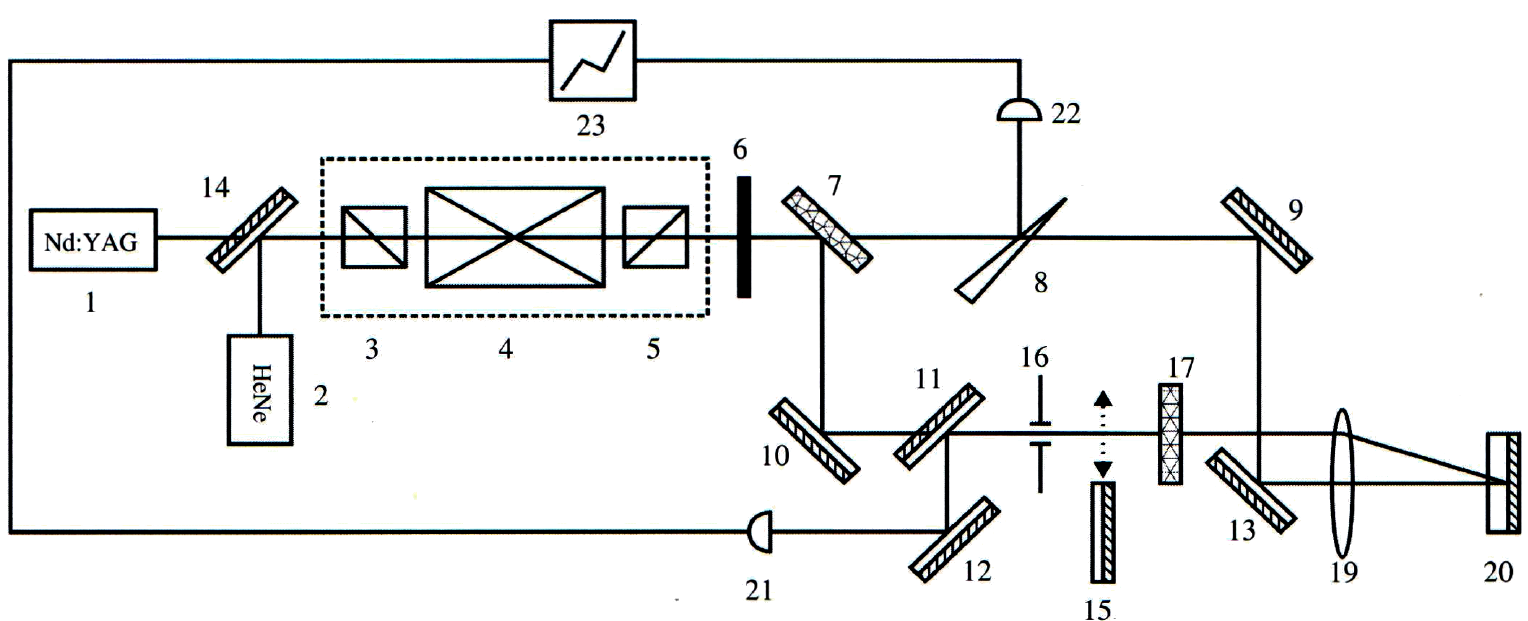
\includegraphics[width=\textwidth]{fig/scheme.png}
	\caption{Схема установки: 1 -- Nd:YAG-лазер; 2 -- НеNе-лазер; 3, 5 -- призмы Глана, 4 -- вращатель Фарадея; 6 -- прерыватель; 7 -- поляризационное зеркало; 8 -- клин; 9-15 -- зеркала; 16 -- диафрагма; 17 -- полуволновая пластинка; 19 -- линза; 20 -- НЖК-ячейка; 21-22 -- фотоприемники; 23 -- осциллограф}
	\label{fig:figure6}
\end{figure}
% Схема оптической части лабораторной установки для наблюдения эффекта ОВФ при четырехволновом смешении представлена на Рис. \ref{fig:figure6}. В комплекте установки находятся непрерывный лазер на алюмоиттриевом гранате с
% неодимом (Nd:YAG), юстировочный гелий-неоновый (Не-Nе) лазер, изолятор
% Фарадея, состоящий из вращателя Фарадея на постоянных магнитах и двух поляризационных призм, кювета с нематическим жидким кристаллом (НЖК),
% зеркала и светоделительные пластины, фотодиоды, электронно-оптический
% преобразователь, регистрирующая аппаратура. Исходный пучок Nd:YAG-лазера \textbf{1} с длиной волны 1.064 мкм мощностью до 0.5 Вт направляется в изолятор Фарадея, а затем модулируется механическим прерывателем \textbf{6}, который формирует импульсы длительностью 0.7 мс.
На рисунке \ref{fig:figure6} представлена схема установки, используемой в данной работе для наблюдения эффекта обращения волнового фронта при четырехволновом смешении. Исходный пучок Nd:YAG-лазера \textbf{1} с длиной волны 1.064 мкм мощностью до 0.5 Вт направляется в изолятор Фарадея\footnote{Изолятор Фарадея за счет эффекта магнитооптического поворота плоскости поляризации, не зависящего от направления распространения излучения, предотвращает попадание встречного плоско-поляризованного пучка в лазер - развязывает лазер и установку}. Из изолятора выходит поляризованное излучение, проходит через прерыватель \textbf{6} (перекрытие излучения с периодом 0.7 с) и становится импульсно-периодическим, после чего поступает на светоделительное поляризационное зеркало \textbf{7}, которое пропускает горизонтально поляризованный компонент пучка -- \textit{пучок накачки} и отражает его вертикально поляризованную составляющую -- \textit{сигнальный пучок}.

Пучок накачки проходит через светоделительный клин \textbf{8}, который отводит небольшую часть накачки (4\%) к фотоприемнику для регистрации мощности, и заводится в НЖК-ячейку толщиной $L=0.5$ см системой зеркал \textbf{9}, \textbf{13} через центр линзы \textbf{20} (фокусное расстояние линзы $F=33$ см). При этом диаметр пучка $a = 0.1$ см.

Сигнальный пучок отражается от зеркала \textbf{10}, проходит через светоделительную пластину \textbf{11}, диафрагму \textbf{16} и полуволновую пластинку \textbf{17}, которая поворачивает плоскость поляризации излучения на 90 градусов.

Светоделительная пластинка \textbf{11} служит для ответвления пучка обращённого излучения, распространяющегося навстречу сигнальном пучку. Обращённый пучок отражается от зеркала \textbf{12} и регистрируется фотоприемником \textbf{21}. Поперечная структура обращенного пучка с помощью осциллографа \textbf{23} сопоставляется со структурой сигнального пучка, излучение которого попадает в \textbf{23} при установке вспомогательного выносного зеркала \textbf{15}.

Сигнальный пучок и пучок накачки фокусируются линзой \textbf{19} в НЖК- ячейку \textbf{20}, где реализуется эффект обращения волнового фронта (ОВФ). НЖК-ячейка \textbf{20} представляет собой плоскопараллельную кювету, в которую заливается жидкий кристалл. Задняя грань кюветы имеет зеркальное покрытие, которое формирует встречную волну накачки.


\newpage
\subsection{Зависимость мощности пучка от тока накачки}
Была получена зависимость мощностей трёх пучков - опорного, сигнального и обращённого от тока накачки диодного лазера. При превышении током накачки порогового значения начинается лазерная генерация, и выходная мощность лазера начинает линейно зависеть от тока накачки. 

В нашем случае можно считать ток и мощность пучка накачки линейно связанными.
\begin{figure}[H]
	\centering
	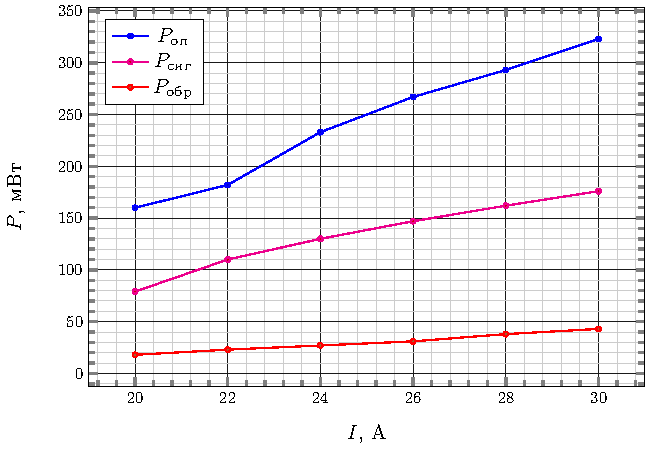
\includegraphics[scale=1.33]{fig/p}
	\caption{Мощность опорного пучка, сигнального и обращённого}
	\label{fig:1}
\end{figure}



\section{Расчёты}
\subsection{Время релаксации}
Сначала оценим значение феноменологического параметра -- коэффициента теплообмена с окружающей средой $\tau_0^{-1}$, исходя из того, что в типичном случае \cite[стр. 19]{met}, когда угол между волновыми векторами сигнальной и опорной волны $\theta \approx 10^{-2}$ рад, длина волны $\lambda \approx 10^{-4}$ см, коэффициент температуропроводности $\chi \approx 10^{-3}$ см${}^2$/сек, время релаксации <<пропускающих>> решеток согласно \eqref{eq:pdv.37} составляет $\tau_\text{r} \approx 10^{-3}$ сек:
\begin{equation}
	\tau_\text{r}=\frac{\tau_{0}}{1+4 \chi \left(\frac{2\pi}{\lambda}\sin{\theta}\right)^{2} \tau_{0}}=
	\frac{\tau_0}{1+4\cdot 10^{-3} \cdot \left(\frac{2\pi}{10^{-4}}\sin{10^{-2}}\right)^{2} \tau_{0}} \approx 10^{-3} \text{ с}
\end{equation}
Решение вышеприведённого уравнения относительно $\tau_0$ даёт $\tau_0 \sim 10^{-3}$ c.

Теперь рассчитаем время релаксации показателя преломления в пропускающей решетке по той же формуле \eqref{eq:pdv.37}, при этом из эксперимента угол между сфокусированными в НЖК-ячейке пучками можно определить через расстояние между пучками в линзе и фокусное расстояние линзы как
\begin{equation}
	\tg \theta = \frac{l}{F} = \frac{5}{330} \quad \rightarrow \quad \theta\approx\frac{l}{F}\approx 1.5\cdot10^{-2},\text{ т.к. } l/F \ll 1.
\end{equation}
При проведении эксперимента было  известно, что $\chi = 10^{-3}$ cм${^2}$/c,  $\lambda = 1064 \cdot 10^{-7}$ см, $\theta \approx 5/330$ рад. Теперь, имея все входящие в время релаксации величины, находим
\begin{equation}
	\tau_\text{r}=\frac{\tau_{0}}{1\!+\!4 \chi \left(\frac{2\pi}{\lambda}\sin{\theta}\right)^{2} \tau_{0}}=
	\frac{10^{-3}}{1\!+\!4\cdot 10^{-3} \cdot \left(\frac{2\pi}{1064\cdot10^{-7}}\sin{(1.5\cdot 10^{-2})}\right)^{2} 10^{-3}} \approx 0.24\cdot10^{-3} \text{ с}.
\end{equation}

\subsection{Проводимость среды}
При распространении волн в жидком кристалле происходит затухание $\sim e^{-2\gamma z}$. Известно, что для используемых жидких кристаллов $\gamma = 1.1$ см$^{-1}$. Потери, обусловленные проводимостью, отражены в  мнимой части комплексной диэлектрической проницаемости
\begin{equation}
	\tilde{\varepsilon} = \varepsilon' + i \varepsilon'' = \varepsilon' - i \frac{4\pi \sigma_0}{\omega}.
\end{equation}
С другой стороны, погонные потери входят в комплексный волновой вектор
\begin{equation}
	\tilde{k} = k' - i\gamma = \frac{\omega}{c}\sqrt{\varepsilon' + i \varepsilon''} = \frac{\omega n}{c}\sqrt{1-i\frac{4\pi \sigma_0}{\omega n^2}},
\end{equation}
где $n = |\sqrt{\varepsilon\mu}| \approx \sqrt{\varepsilon'} = 1.5$. В случае малых потерь, а именно в этом приближении получен коэффициент отражения \eqref{eq:2.68}, можно разложить $\tilde{k}$ в ряд по малому параметру $p=4\pi\sigma_0 / \omega n^2$
\begin{equation}
	\tilde{k} = n\frac{\omega}{c} - \frac{i n\omega}{2c} \frac{4\pi \sigma_0}{\omega n^2} + o(p^2).
\end{equation}
Отбрасывая члены ряда с вторым и выше порядком малости, приближенно получаем
\begin{equation}
	\gamma \approx \frac{2\pi \sigma_0}{nc},
\end{equation}
откуда выражаем удельную проводимость через коэффициент затухания
\begin{equation}
	\sigma_0 \approx \frac{\gamma n c}{2\pi} = \frac{1.1\text{ см}^{-1} \cdot 1.5 \cdot 2.99\cdot 10^{10}\, \frac{\text{см}}{\text{с}}}{2\pi} = 0.785\cdot 10^{10} \text{ с}^{-1},
\end{equation}
что в единицах СИ имеет порядок $1$ См/м. Это небольшая проводимость: на 7 порядков меньше проводимости металлов, таких как медь или серебро. 

\subsection{Интенсивность пучка накачки}
Основная  мода используемого в данной работе Nd:YAG лазера -- TEM${}_{00}$. Эта мода имеет  гауссово поперечное распределение амплитуды электрического поля
\begin{equation}
	\vec{E}=\vec{E}_{0} \exp\left(-\frac{r^2_\perp}{2 a^2}\right).
\end{equation}
Найдём полную мощность пучка накачки $P_\text{оп}$  как поток вектора Пойнтинга (будем далее подразумевать под вектором Пойнтинга -- его среднее за период значение) через сечение пучка:
\begin{equation}
	P_\text{оп} = \iint \vec{S} \, \mathrm{d}{\vec{\sigma}} = 
	\int\limits_0^\infty \frac{c}{8\pi}\sqrt{\frac{\varepsilon_0}{\mu}}{|\vec{E}|^2}\cdot 2\pi r_\perp \, \mathrm{d}r_\perp=
\end{equation}
\begin{equation}
	=\int\limits_0^\infty \frac{nc}{8\pi}\cdot |\vec{E}_0|^2\exp\left(-\frac{r^2_\perp}{a^2}\right) \cdot 2\pi r_\perp \, \mathrm{d}r_\perp=\left[x=\frac{r^2_\perp}{a^2},\,\,\,\mathrm{d}r_\perp = \frac{a}{\sqrt{x}}\mathrm{d}x\right]=
\end{equation}
\begin{equation}
	=\frac{nc}{4}\cdot\frac{|\vec{E}_0|^2 a^2}{2}\int\limits_0^\infty e^{-x} \, \mathrm{d}x  = \frac{a^2 nc}{8} |\vec{E}_0|^2 = \frac{a^2I_0 nc}{8}
	\quad \Rightarrow \quad I_0 = \frac{8P_\text{оп}}{a^2 nc}.
\end{equation}
В эксперименте были получены значения мощности измеряемого калориметром пучка накачки от 150 до 323 мВт. При этом необходимо учесть, что измеряется мощность модулированного меандром (скважность 2) пучка, и следовательно измеряемая  средняя мощность в два раза ниже мощности пучка (средней за время открытия обтюратора)   
\begin{equation}
	P_\text{оп} = 2P_\text{оп}^\text{изм}.
\end{equation}
Найдём интенсивность при характерной в данном эксперименте мощности пучка накачки 400 мВт:
\begin{equation}
	I_0 = \frac{8\cdot 0.4 \cdot 10^7\, \frac{\text{эрг}}{\text{с}}}{(0.1\text{ см})^2 \cdot 1.5 \cdot 3\cdot 10^{10}  \,\frac{\text{см}}{\text{с}}}=0.71 \,\frac{\text{эрг}}{\text{см}^3}.
\end{equation}

\subsection{Коэффициент нелинейности}
Найдём значение безразмерного коэффициента нелинейности среды по формуле \eqref{eq:pdv.39}. Подставим ранее рассчитанные значения интенсивности пучка накачки $I_0 = 0.71 \,\frac{\text{эрг}}{\text{см}^3}$, проводимости нелинейной среды $\sigma_0 = 0.785\cdot 10^{10} \text{ с}^{-1}$, время релаксации $\tau_\text{r} = 0.24\cdot 10^{-3}$ с, известные заранее значения диэлектрической проницаемости $\varepsilon_0 = n^2 = 1.5^2$, произведение плотности и теплоёмкости при постоянном давлении $\rho_0 C_p\approx 10^7$ эрг/см${}^3$К, $\qty(\pdv{\varepsilon}{T})_p\approx 10^{-3}$ K${}^{-1}$:
\begin{equation}
	\label{eq:exp.pdv.39}
	G = \frac{\sigma_0 \tau_\text{r} I_0}{4 \varepsilon_0 \rho_0 C_p} \left(\frac{\partial \varepsilon}{\partial T}\right)_p = 
	\frac{0.785\cdot 10^{10} \cdot 0.24\cdot10^{-3} \cdot 0.71}{4\cdot {1.5}^2\cdot 10^7}\cdot 10^{-3} = 1.48\cdot 10^{-5}.
\end{equation}


\subsection{Коэффициент отражения}
Найдем значение коэффициента отражения (по мощности) по формуле \eqref{eq:2.68}
\begin{equation}
	\label{eq:exp.2.68}
	r^{2}=\operatorname{tg}^{2}(G L'),
\end{equation}
где $L'$ -- безразмерная толщина НЖК-ячейки. Размерная длина $L=0.5$ см известна, безразмерная же находится преобразованием координат \eqref{eq:pdv.35}
\begin{equation}
	L' = L \cdot \frac{k^2}{k_z \varepsilon_0} = 0.5 \cdot \frac{2\pi / (1064\cdot10^{-7})}{\cos{(1.5\cdot10^{-2})}{1.5}^2} = 19653.
\end{equation}
Тогда можем найти значение коэффициента отражения зеркала 
\begin{equation}
	r^2 = \operatorname{tg}^{2}(19653 \cdot 1.48\cdot 10^{-5})=0.30.
\end{equation}

Для разных входных мощностей (токов накачки) посчитаны значения коэффициента отражения $r^2 = \tg^2(G\cdot L')$. Полученные значения  предоставлены на графике ниже.
\begin{figure}[H]
	\centering
	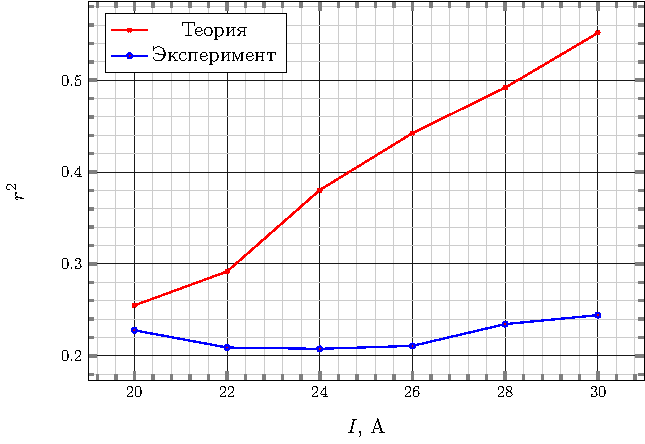
\includegraphics[scale=1.33]{fig/r}
	\caption{Коэффициент отражения}
	\label{fig:2} 
\end{figure}

Как видно, теоретическое значение коэффициента отражения растет с ростом накачки, что отвечает связи $r \sim \tg P$.  В ходе эксперимента получены значения меньшие, чем предсказывала теория. Это может быть обусловлено особенностями реализации эксперимента: например, возникновение при нагреве активной среды лазера тепловой линзы, что приводит к появлению паразитных мод в лазере и увеличению угла расходимости лазерного пучка. Недостаточная термостабилизация элементов установки может привести к разбросу характеристик, таких как длина генерируемой волны, мощность пучка - и в итоге частично подавлять ОВФ-эффект.

% \newpage
\addcontentsline{toc}{section}{Заключение}
\section*{Заключение}
В настоящей работе мы изучили метод преобразования излучения четырехволновым взаимодействием, рассчитали коэффициент отражения ОВФ-зеркала, получили зависимости мощностей трех пучков от тока накачки. Качественно наблюдается рост коэффициента ОВФ-отражения при росте мощности накачки, хотя количественно теоретическое значение больше. Можно предположить, что такой результат получается из-за  неидеальности лабораторных условий, приводящих к возникновению побочных эффектов -- таких, как искажение модового состава лазерного излучения, увеличение угла пучка излучения и т.п. 

\begin{thebibliography}{}
  \bibitem{met} Миловский Н.\,Д., Мартынова О.\,В., Зиновьев А.\,П. Преобразование лазерного излучения методами нелинейной оптики: методическое пособие. -- Нижний Новгород: Нижегородский государственный университет им. Н.И. Лобачевского, 2014. -- 38 с.
    
\end{thebibliography}
\end{document}




